% concatenated from symmetric.tex
\documentclass[12pt]{article}

%\setlength\parindent{0pt}

\usepackage{geometry}
\usepackage{amsmath,amssymb,amsthm,comment,enumitem, array}
\usepackage{color}
\usepackage{parskip}
\usepackage{parskip}
\usepackage{setspace}
\usepackage{graphicx}
\usepackage{mathtools}
\usepackage{subfig}
\usepackage{comment}
\usepackage{mathabx}
\usepackage{mathrsfs}
\usepackage{setspace}
\usepackage{bm}
\usepackage[normalem]{ulem}
\usepackage{cancel}
\usepackage{csquotes}
%\usepackage{biblatex}
\usepackage[colorlinks=true, allcolors=blue]{hyperref}
\hypersetup{colorlinks, citecolor=red, filecolor=black, linkcolor=blue, urlcolor=blue}
\usepackage{pgfplots}
\pgfplotsset{compat=1.18}
\usepackage{graphics}
\usepackage{graphicx}
\usepackage{tikz}
\usepackage{circuitikz}
\usepackage{tcolorbox}
\usepackage{enumitem}
\usepackage{subfiles}
\usepackage{ytableau}
\usepackage{thmtools}
\usepackage{thm-restate}
\usepackage{multicol}

\newcommand\s{\mathcal}
\newcommand\sss{\mathscr}
\newcommand\ov{\overline}
\newcommand\bo{\textbf}
\newcommand\bb{\mathbb}
\newcommand\PP{\bb{P}}
\newcommand\EE{\bb{E}}
\newcommand\II{\bb{I}}
\newcommand\NN{\bb{N}}
\newcommand\FF{\bb{F}}
\newcommand\RR{\bb{R}}
\newcommand\QQ{\bb{Q}}
\newcommand\CC{\bb{C}}
\newcommand\ZZ{\bb{Z}}
\newcommand\ra{\Longrightarrow}
\newcommand\lra{\Longleftrightarrow} 
\newcommand\code{\texttt}
\newcommand\lb{\langle} 
\newcommand\rb{\rangle} 
\newcommand\ti{\Tilde} 
\newcommand\Var{\text{Var}} 
\newcommand\Cov{\text{Cov}} 
\newcommand\Cor{\text{Cor}} 
\newcommand\Span{\text{Span}} 
\newcommand\sm{\setminus}
\newcommand\Spec{\text{Spec}}
\newcommand\Inn{\text{Inn}}
\newcommand\wh{\widehat}
\newcommand\diam{\text{diam}}
\newcommand\ns{\text{null}}
\newcommand\diag{\text{diag}}
\newcommand\dnd{\nmid}
\newcommand\Ker{\text{Ker}}
\newcommand\lcm{\text{lcm}}
\newcommand\Gal{\text{Gal}}
\newcommand\ch{\text{char}}
\newcommand\per{\text{per}}
\newcommand\Aut{\text{Aut}}
\newcommand\Fix{\text{Fix}}
\newcommand\cl{\text{cl}}
\newcommand\TT{\mathbb{T}}
\newcommand\ex{\mathrm{ex}}
\newcommand\EX{\mathrm{EX}}
\newcommand\sgn{\mathrm{sgn}}
\newcommand\proj{\mathrm{proj}}
\newcommand\comp{\mathrm{comp}}
\newcommand\curl{\mathrn{curl}}
\newcommand\dive{\mathrm{div}}
\newcommand{\norm}[1]{\left \lVert #1 \right \rVert}

\newtheorem{thm}{Theorem}
\newtheorem{defn}{Definition}
\newtheorem{lemma}{Lemma}
\newtheorem{prop}{Proposition}
\newtheorem{claim}{Claim}
\newtheorem{rmk}{Remark}
\newtheorem{eg}{Example}
\newtheorem{prob}{Problem}
\newtheorem{cor}{Corollary}
\newtheorem{fact}{Fact}
\newtheorem{exe}{Exercise}
\newtheorem{conj}{Conjecture}
\newtheorem{quest}{Question}

\def\john#1{\noindent
\textcolor{green}
{\textsc{(John:}
\textsf{#1})}}

\def\mike#1{\noindent
\textcolor{red}
{\textsc{(Mike:}
\textsf{#1})}}

%\addbibresource{references.bib}

\title{New constructions and bounds for nonabelian Sidon sets with applications to Tur\'an-type problems}
\author{John Byrne\thanks{Department of Mathematical Sciences, University of Delaware. \texttt{jpbyrne@udel.edu}} \and Michael Tait\thanks{Department of Mathematics \& Statistics, Villanova University. \texttt{michael.tait@villanova.edu}. Both authors were partially supported by NSF grant DMS-2245556}}
\date{\today}

\begin{document}
\maketitle

\begin{abstract}
    An $S_k$-\textit{set} in a group $\Gamma$ is a set $A\subseteq\Gamma$ such that $\alpha_1\cdots\alpha_k=\beta_1\cdots\beta_k$ with $\alpha_i,\beta_i\in A$ implies $(\alpha_1,\ldots,\alpha_k)=(\beta_1,\ldots,\beta_k)$. An $S_k'$-\textit{set} is a set such that $\alpha_1\beta_1^{-1}\cdots\alpha_k\beta_k^{-1}=1$ implies that there exists $i$ such that $\alpha_i=\beta_i\text{ or }\beta_i=\alpha_{i+1}$. We give explicit constructions of large $S_k$-sets in the group $S_n$ and $S_2$-sets in $S_n\times S_n$ and $A_n\times A_n$. We give probabilistic constructions for `nice' groups which obtain large $S_2$-sets in $A_n$ and $S_2'$-sets in $S_n$. We also give upper bounds on the size of $S_k$-sets in certain groups, improving the trivial bound by a constant multiplicative factor. We describe some connections between $S_k$-sets and extremal graph theory. In particular, we determine up to a constant factor the minimum outdegree of a digraph which guarantees even cycles with certain orientations. As applications, we improve the upper bound on Hamilton paths which pairwise create a two-part cycle of given length, and we show that a directed version of the Erd\H{o}s-Simonovits compactness conjecture is false.
\end{abstract}

\section{Introduction} \label{Introduction}

\subsection{Background}

A \textit{Sidon sequence} in $[n]$ is a subset $A\subseteq\mathbb N$ such that the pairwise sums $a+b$ with summands taken from $A$ are all different, i.e.
$$\forall a,b,c,d\in A\,  a+b=c+d\Longrightarrow\{a,b\}=\{c,d\}.$$
This notion was introduced by Sidon \cite{sidon1932satz} in his work on Fourier analysis. Erd\H{o}s and Tur\'an \cite{erdos1941problem} proved that the maximum size $\Phi(n)$ of a Sidon sequence in $[n]$ satisfies $(1/\sqrt 2-o(1))\sqrt n<\Phi(n)<(1+o(1))\sqrt n$ and it was later shown that $\Phi(n) \sim \sqrt{n}$ \cite{bosechowla}. Since then many variants and generalizations of this problem have been studied and there is great interest in bounding the maximum size of a Sidon set in a given group. For further reading we refer to \cite{bajnok2018additive} and \cite{o2004complete}.

In this paper we are concerned with Sidon sets and their generalizations in arbitrary, possibly nonabelian groups, which were introduced by Babai and S\'os \cite{babai1985sidon}:

\begin{defn}
    Let $\Gamma$ be a group. We say that $A\subseteq\Gamma$ is a \textit{Sidon set of the first kind} if
    $$\alpha\beta=\gamma\delta$$
    with $\alpha,\beta,\gamma,\delta\in A$ implies that $|\{\alpha,\beta,\gamma,\delta\}|\le 2$. We say that $A$ is a \textit{Sidon set of the second kind} if
    $$\alpha\beta^{-1}=\gamma\delta^{-1}$$
    with $\alpha,\beta,\gamma,\delta\in A$ implies $|\{\alpha,\beta,\gamma,\delta\}|\le 2$. 
\end{defn}

Observe that if $\Gamma$ is abelian then these two conditions are equivalent. The authors of \cite{babai1985sidon} used probabilistic methods to construct large Sidon sets of both kinds in general groups.

\begin{thm}[Babai-S\'os \cite{babai1985sidon}] \label{Babai Sos lower bound}
Let $\Gamma$ be a group and $W\subseteq\Gamma$ be finite. Then $W$ contains Sidon sets of both kinds, of size
$(c+o(1))|W|^{1/3}$, where $c=3\cdot2^{1/3}/8>0.47247$.
\end{thm}
Godsil and Imrich \cite{godsil1987embedding} improved the constant to $(2/(7+4\sqrt 3))^{1/3}> 0.52365$ for Sidon sets of the first kind and $1/(2+\sqrt 3)^{1/3}>0.64468$ for Sidon sets of the second kind.

If $\Gamma$ is abelian, we say $A\subseteq\Gamma$ is a $B_k[g]$-set ($B_k$-set if $g=1$) if for any $\mu\in\Gamma$, there is at most one multiset $\{\alpha_1,\ldots,\alpha_k\}$ with $\alpha_i\in A$ such that $\alpha_1+\cdots+\alpha_k=\mu$. Odlyzko and Smith \cite{odlyzko1995nonabelian} introduced the following non-abelian analogue of $B_k$-sets.

\begin{defn}
    Let $\Gamma$ be a group. We say $A\subseteq\Gamma$ is a (nonabelian) $S_k$-set if whenever $$\alpha_1\cdots\alpha_k=\beta_1\cdots\beta_k$$
    with $\alpha_i,\beta_i\in A$, we have
    $$(\alpha_1,\ldots,\alpha_k)=(\beta_1,\ldots,\beta_k).$$
\end{defn}

An $S_2$-set is a Sidon set of the first kind but the converse is not  necessarily true. One may generalize $S_k$-sets to a nonabelian analogue of $B_k[g]$-sets:

\begin{defn}
    Let $\Gamma$ be a group. We say $A\subseteq\Gamma$ is an $S_k[g]$-set if for any $\mu\in\Gamma$ there are at most $g$ words $(\alpha_1,\ldots,\alpha_k)$ such that $\alpha_1\cdots\alpha_k=\mu$.
\end{defn}

Note that $\Gamma$ being nonabelian allows us to impose the stronger condition of the equality of the words $(\alpha_1,\ldots,\alpha_k)$ and $(\beta_1,\ldots,\beta_k)$ rather than of the multisets $\{\alpha_1,\ldots,\alpha_k\}$ and $\{\beta_1,\ldots,\beta_k\}$. This is important for the applications of Sidon-type sets to extremal graph theory. Given a set $A\subseteq\Gamma$, its \textit{Cayley graph} $\mathrm{Cay}(\Gamma,A)$ is the digraph with vertex set $\Gamma$ where $\alpha\beta$ is an edge whenever $\alpha^{-1}\beta\in A$; its \textit{bipartite Cayley graph} $\mathrm{BCay}(\Gamma,A)$ is the undirected graph with vertex set $\Gamma\times\{0,1\}$ whose edges are $\{(\alpha,0),(\alpha\beta,1)\}$ for $\alpha\in\Gamma,\beta\in A$. It is well-known that the bipartite Cayley graph of a $B_2$-set is $C_4$-free: see \cite{tait2013sidon,daza2018sidon} for applications of this connection to extremal graph theory. Unfortunately, when $k\ge 3$ the bipartite Cayley graph of a $B_k$-set contains a $C_{2k}$. However, as described in \cite{odlyzko1995nonabelian} there is hope of constructing large $C_{2k}$-free graphs using another non-abelian analogue of $B_k$-sets.

\begin{defn}
    Let $\Gamma$ be a group. We say $A\subseteq\Gamma$ is an $S_k'$-set if whenever
    $$\alpha_1\beta_1^{-1}\cdots\alpha_k\beta_k^{-1}=1$$
    with $\alpha_i,\beta_i\in A$, we have for some $i$ that $\alpha_i=\beta_i$ or $\beta_i=\alpha_{i+1}$. 
\end{defn}

An $S_2'$-set is a Sidon set of the second kind but the converse is not true. However, observe that the bipartite Cayley graph of an $S_k'$-set is $C_{2k}$-free. A partial converse holds: if $G$ is a (bipartite) Cayley graph with girth greater than $2k$, then the generating set is an $S_k'$-set. This means that constructions of high-girth Cayley graphs can be phrased in terms of $S_k'$-sets; for example, the Ramanujan graphs of Lubotzky, Phillips, and Sarnak \cite{lubotzky1988} provide a construction of $S_k'$-sets in $\mathrm{PSL}(2,q)$ and $\mathrm{PGL}(2,q)$.

Let $M_{k,g}(\Gamma)$ denote the maximum size of an $S_k[g]$-set in $\Gamma$, and let $M_k'(\Gamma)$ denote the maximum size of a $S_k'$-set in $\Gamma$. When $g=1$, we just write $M_k(\Gamma)$. If $A$ is an $S_k$-set then the words in $A^k$ give distinct products, so we have the trivial upper bound $M_k(\Gamma)\le|\Gamma|^{1/k}$. More generally, $M_{k,g}(\Gamma)\le (g|\Gamma|)^{1/k}$. For $S_k'$-sets the general upper bound is not so immediate. Let $A\subseteq\Gamma$ be an $S_k'$-set. Then $\mathrm{BCay}(\Gamma,A)$ is a $C_{2k}$-free graph on $2|\Gamma|$ vertices with $|\Gamma||A|$ edges. The even cycle theorem \cite{bondy1974cycles} gives $|\Gamma||A|=O(|\Gamma|^{1+1/k})$, so $M_k'(\Gamma)=O(|\Gamma|^{1/k})$. The authors of \cite{odlyzko1995nonabelian} constructed $S_k$-sets in certain infinite families of groups whose size is within a constant factor of the upper bound:

\begin{thm}[Odlyzko-Smith \cite{odlyzko1995nonabelian}] \label{Odlyzko result}
For each integer $k$ at least $2$, and any prime $p$ with $k|(p-1)$, a nonabelian group $G$ of order $|G|=(p^k-1)k$ exists which contains a nonabelian $S_k$-set $S$ of cardinality $(p-1)/k$.
\end{thm}

Our aims in this paper are twofold. First, we give lower and upper bounds on $M_k(\Gamma)$ and $M_k'(\Gamma)$ in various groups. We list these results in \autoref{Subsection Sidon sets}. Second, we establish connections between $S_k$-sets and some problems in extremal graph theory, and we study these problems in their own right. We list these results in \autoref{Subsection extremal graph theory}.

\subsection{Results on Sidon sets} \label{Subsection Sidon sets}

Our lower bounds on $M_k(\Gamma)$ will focus on the groups $S_n,S_n\times S_n$, and $A_n\times A_n$, where $S_n$ and $A_n$ are the symmetric and alternating groups on $n$ letters, respectively. There is a large literature on extremal problems for the symmetric group, including properties of its Cayley graphs. For example, Helfgott and Seress \cite{helfgott2014diameter} showed that if $\Gamma=S_n$ or $\Gamma=A_n$ then for any set $A\subseteq\Gamma$ which generates $\Gamma$, every element of $\Gamma$ can be expressed as a product of $\mathrm{exp}((\log\log|\Gamma|)^{O(1)})$ elements of $A\cup A^{-1}$. Keevash and Lifshitz \cite{KL} obtained results on combinatorial properties of the symmetric group, including diameter of the Cayley graph of a dense generating set and the size of subsets avoiding the equation $\alpha\beta=\gamma^2$. Recently Keevash, Lifshitz, and Minzer \cite{KLM} determined the maximum product-free subsets of $A_n$. Illingworth, Michel, and Scott \cite{IMS} studied similar problems in infinite groups. Our first result is a lower bound on $M_k(S_n)$.


\begin{comment} This is for two reasons. First, certain tools apply only to the symmetric group, namely the Egorychev-Falikman theorem bounding the permanent of a matrix and the description of conjugacy in $S_n$. Second, we will prove in \autoref{Sk' upper bound} and \autoref{Sk upper bound} that $S_k'$ sets (and $S_k$-sets when $k$ is even) of close to optimal size can only exist when $\Gamma$ has no large abelian subgroups. Thus, it makes sense to ensure that the largest nonabelian subgroup has order $|\Gamma|^{o(1)}$.\end{comment} 

\begin{thm} \label{Sk sets in Sn lower bound} For all $k$, we have
$$M_k(S_n)=(n!)^{1/k+O(1/\log n)}.$$
\end{thm}

The idea of \autoref{Sk sets in Sn lower bound} is to use the $S_k$-sets of \autoref{Odlyzko result} and consider the permutations of $\Gamma$ which map each $\alpha$ to some $\alpha\beta$, where $\beta$ belongs to the $S_k$-set. The Egorychev-Falikman theorem \cite{egorychev,falikman}, which provides a lower bound on the permanent of a doubly stochastic matrix, allows us to estimate the number of such permutations. 

Observe that if $A_1\subseteq\Gamma_1$ and $A_2\subseteq\Gamma_2$ are $S_k$-sets, then $A_1\times A_2$ is an $S_k$-set in $\Gamma_1\times\Gamma_2$. This is a notable contrast to $B_k$-sets. As a consequence, \autoref{Sk sets in Sn lower bound} gives that $M_k(S_n\times S_n)\ge(n!)^{2/k-O(1/\log n)}.$ In the case $k=2$, we provide a better construction whose size can be computed exactly and which is optimal up to a factor of $n$.

\begin{thm} \label{Sn times Sn result}
    For every $n$ we have
    \begin{itemize}
        \item[(a)] $M_2(S_n\times S_n)\ge(n-1)!$
        \item[(b)] $M_{2,n}(S_n\times S_n)\ge n!$
        \item[(c)] $M_2(A_n\times A_n)\ge(n-1)!/2$
        \item[(d)] $M_{2,n}(A_n\times A_n)\ge n!/2.$
    \end{itemize}
\end{thm}

Inspired by the construction of Sidon sets in elementary abelian groups of order $q^2$ \cite{lindstrom1969determination,babai1985sidon} (which are themselves based on the original construction of Erd\H{o}s and Tur\'an \cite{erdos1941problem}), our constructions are loosely of the form $\{(\alpha,f(\alpha)):\alpha\in\Gamma\}$ where $f:\Gamma\to\Gamma$. However, in nonabelian groups we cannot use polynomials so we require other tools to find a function $f$ which gives a Sidon set. In the case of $S_n$ we are able to exploit the relationship between cycle structure and conjugacy. \autoref{Sk sets in Sn lower bound} and \autoref{Sn times Sn result} give not only an explicit construction of $S_2$-sets in these groups but also, to our knowledge, the first improvement over \cite{godsil1987embedding} on Sidon sets of the first kind in these groups. In \autoref{Conjugacy section} we also generalize parts (b) and (d) of \autoref{Sn times Sn result} to any group with a large conjugacy class.

We also consider Sidon sets of the second kind in $S_n$. Unfortunately, neither the idea of \autoref{Sk sets in Sn lower bound} nor its graph-theoretic generalization work here. That is, taking permutations from a $C_4$-free graph does not give rise to a Sidon set of the second kind in any direct way (see \autoref{Concluding remarks} for details). We make do with a general probabilistic lower bound, extending \autoref{Babai Sos lower bound} to $S_2$-sets and $S_2'$-sets. We did not attempt to optimize the constants.

\begin{comment}Instead, we obtain the following result which gives a relation between Sidon sets of the second kind and a new extremal problem on permutations.

\begin{prop} \label{second kind result}
    Let $G$ be a balanced $C_4$-free bipartite graph on $2n$ vertices with $m$ perfect matchings. Then there exists $A\subseteq S_n$ with $|A|=m$ such that for all $\alpha,\beta,\gamma,\delta\in A$
    \begin{equation} \label{sidon implication}
    \alpha\beta^{-1}=\gamma\delta^{-1}\Longrightarrow\forall i\ [\alpha(i)=\beta(i)\text{ and }\gamma(i)=\delta(i)]\text{ or }[\alpha(i)=\gamma(i)\text{ and }\beta(i)=\delta(i)].
    \end{equation}
\end{prop}

In particular, for all $i$ $|\{\alpha(i),\beta(i),\gamma(i),\delta(i)\}|\le 2$, motivating the following definition.

\begin{defn}
    We say that $A\subseteq S_n$ is a $t$-wise $v$-value set  $\pi_1,\ldots,\pi_t\in A$,
    $$\exists i\ |\{\pi_1(i),\ldots,\pi_t(i)\}|\ge v.$$
    We write $\Delta^t_v(n)$ for the maximum size of a $t$-wise $v$-value set in $S_n$.
\end{defn}

Our interest in \autoref{second kind result} comes from the observation that if $A$ is a set satisfying \autoref{sidon implication} and $B$ is a 4-wise 3-value set then $A\cap B$ is a Sidon set of the second kind. This gives the following corollary.

\begin{cor} \label{second kind lower bound} There exists an $S_2'$-set in $S_n$ of size at least
$$(n!)^{1/2-O(1/\log n)}\cdot\frac{\Delta_3^4(n)}{n!}.$$
\end{cor}

Motivated by \autoref{second kind lower bound}, we present some results on $t$-wise $v$-value sets.

\begin{thm} \label{v value sets}
    We have for any fixed $t\ge v$:
    \begin{itemize}
        \item[(a)] $\Delta^{t+1}_{v+1}(n)\le \Delta^t_v(n)\le \Delta^{t+1}_v(n)$
        \item[(b)] $(n!)^{1-(v-2)/(t-1)-O(1/\log n)}\le \Delta^t_v(n)\le\frac{(t-1)n!}{(v-1)!^{\lfloor n/(v-1)\rfloor}}$
    \end{itemize}
\end{thm}

The functions $\Delta^t_v$ are related to $q-$ary $k-$hash codes, defined as subsets $A\subseteq[n]^q$ such that any $k$ of them all differ in some coordinate. Specifically, $\Delta^t_t(n)$ is at most the maximum size of an $n$-ary $t$-hash code of length $n$. Blackburn and Wild \cite{blackburn1998optimal} presented an upper bound on the size of hash codes implying that $\Delta^t_t(n)\le(n!)^{1/(t-1)+O(1/\log n)}$, which meets the lower bound in \autoref{v value sets} for $t=v$. It is not clear to us whether their argument can be generalized to the case $t>v$. 
%There is also the notion of separating hash families \cite{stinson2008generalized} which comes closer to our $t$-wise $v$-value sets but it seems the relationship is also in the wrong direction to improve our bounds. 

One can also drop the requirement that the code consists of permutations and consider the maximum size $D^t_v(n,q)$ of a set of words in $[q]^n$ any $t$ of which have at least $v$ different values in some coordinate. This function is interesting even with $n$ fixed and $q\to\infty$, for example one can show that $D^4_3(2,q)$ equals the Zarankiewicz number $z(q,q;2,2)$. We note that a relationship between perfect hash families and hypergraph Tur\'an problems has been observed in \cite{shangguan2016separating}.

\autoref{v value sets} gives the lower bound $\Delta^4_3(n)\ge(n!)^{2/3-O(1/\log n)}$ which combined with \autoref{second kind lower bound} gives $M_2'(S_n)\ge(n!)^{1/6-O(1/\log n)}.$ However, the exponent of $1/6$ is not optimal, as shown by a direct probabilistic construction. \end{comment}

\begin{prop} \label{Probabilistic constructions}
We have the following lower bounds on $M_2(\Gamma)$ and $M_2'(\Gamma)$.
\begin{itemize}
    \item[(a)] Suppose that a group $\Gamma$ has a set $B$ of size $b$ where any distinct $\beta_1,\beta_2\in B$ satisfy $\beta_1^2\ne\beta_2^2$ and $\beta_1\beta_2\ne\beta_2\beta_1$. Then $M_2(\Gamma)\ge(0.39+o(1))b^{1/3}.$
    \item[(b)] Suppose $\Gamma$ has exactly $i$ involutions. If $i=o(|\Gamma|^{2/3})$, then $M_2'(|\Gamma|)\ge (0.39+o(1))|\Gamma|^{1/3}$. If $i=\Omega(|\Gamma|^{2/3})$, then $M_2'(\Gamma)=\Omega(|\Gamma|/i)$.
\end{itemize}
\end{prop}

We give two applications. First, we note that $S_n$ has $(n!)^{1/2+o(1)}$ involutions, so \autoref{Probabilistic constructions} (b) gives $M_2'(S_n)=\Omega(n!^{1/3})$. By taking translations it follows that also $M_2'(A_n)=\Omega(n!^{1/3})$. Second, we consider $M_2(A_n)$. Let $B$ be a set of $n$-cycles or $(n-1)$-cycles fixing the same element (so that their sign is even) where $\pi\in B\Longrightarrow\pi^k\not\in B$ for $k\ne 1$. We can always find at least $(n-2)!/n$ such cycles. Since the sign of the cycles is even, we have $\beta_1^2\ne\beta_2^2$ for $\beta_1,\beta_2\in B$. It is well-known that two cycles $\pi,\sigma$ commute if and only if they are disjoint or $\sigma\in\lb\pi\rb$. Thus, $\beta_1\beta_2\ne\beta_2\beta_1$ for $\beta_1,\beta_2\in B$. Therefore, $M_2(A_n)\ge(n!)^{1/3-o(1)}$. To our knowledge these lower bounds are the best known, although we suspect the correct exponent is $1/2-o(1)$ in both cases.

We note that, in general, it is harder to give probabilistic lower bounds for $S_k$-sets or $S_k'$-sets than for Sidon sets. For example, the largest number $b$ attainable for \autoref{Probabilistic constructions} (a) can vary between 1 and $|\Gamma|^{1-o(1)}$ depending on the structure of the group. 

Finally we present upper bounds on the size of $S_k$-sets and $S_k'$-sets. Dimovski \cite{dimovski1992groups} proved that equality can never hold in the trivial bound on $S_k$-sets, i.e. $M_k(\Gamma)<|\Gamma|^{1/k}$
whenever $|\Gamma|>1$. Our main upper-bound result generalizes the argument of \cite{dimovski1992groups} to show that a kind of stability sometimes holds.

\begin{thm} \label{Sk upper bound}
    For any $h$ and any even $k$, there is $\varepsilon>0$ such that any sufficiently large group $\Gamma$ containing a normal abelian subgroup $H$ with $|\Gamma:H|=h$ satisfies
    $$M_k(\Gamma)\le(1-\varepsilon)|\Gamma|^{1/k}.$$
\end{thm}

In \autoref{Upper bound section} we prove various other upper bounds on $M_k(\Gamma)$ and $M_k'(\Gamma)$ when some information about the structure of $\Gamma$ is known.

\subsection{Results on extremal graph theory} \label{Subsection extremal graph theory}

Our first result in this category demonstrates another connection between Sidon sets and extremal graph theory, in the `reverse' direction: given a $C_{2k}$-free graph on $n$ vertices, one can construct an $S_k$-set in $S_n$.

\begin{thm} \label{hamilton cycles result}
    Suppose $G$ is a graph on $n$ vertices with girth at least $2k+1$ that contains $h$ Hamilton cycles. Then $M_k(S_n)\ge h/2^{n-1}$.
\end{thm}

Note that \autoref{hamilton cycles result} never improves \autoref{Sk sets in Sn lower bound} and only provides an equally good bound in the cases $k=2,3,5$ (in these cases, one can use pseudorandom constructions of extremal high-girth graphs to count the Hamilton cycles, see \cite{byrne2024improved}). However we find the result to be interesting for two reasons. First, it demonstrates that the connection between additive combinatorics and $C_{2k}$-free graphs sometimes goes in both directions. Second, it potentially implies the existence of many more distinct maximal $S_k$-sets than is guaranteed by \autoref{Sk sets in Sn lower bound}, owing to the increased flexibility of graphs as compared with Sidon sets. 

Next we consider the relationship between $S_k$-sets and directed graphs. Some terminology is required: let $\mathcal F_k$ be the set of all digraphs which are the union of two distinct directed walks of length $k$ with the same initial and same terminal vertices, let $C_{k,k}$ be the graph consisting of two vertices $x,y$ joined by two internally disjoint paths on $k$ edges, each oriented from $x$ to $y$, and let $\mathcal C_{k,k}=\{C_{2,2},\ldots,C_{k,k}\}$. If $\mathcal F$ is a family of (directed) graphs then $\mathrm{ex}(n,\mathcal F)$ is the maximum number of edges in a (directed) graph with no subgraph isomorphic to $\mathcal F$.

Huang and Lyu \cite{huang2020extremal} showed that $\mathrm{ex}(n,C_{2,2})=n^2/4+n+O(1)$ and determined the extremal digraphs for $n\ge 13$. Later \cite{huang2024extremal}, they determined $\mathrm{ex}(n,F)$ for large $n$ where $F$ is a particular orientation of $\Theta_{\ell,\ldots,\ell}$, in particular $\mathrm{ex}(n,C_{\ell,\ell})=n^2/4+O(n)$. Wu \cite{wu20100} showed that $\mathrm{ex}(n,\mathcal F_2)=n^2/4+n+O(1)$ and determined the extremal digraphs. Huang, Lyu, and Qiao \cite{huang2019turan} showed that for $k\ge 4$, $\mathrm{ex}(n,\mathcal F_k)=n^2/2-\lfloor n/k\rfloor^2/2+O(n)$ and determined the extremal digraphs when $k\ge 5$ and $n\ge k+5$. Huang and Lyu \cite{huang2022extremal} showed that $\mathrm{ex}(n,\mathcal F_3)=\lfloor n^2/3\rfloor+1$ and determined the extremal digraphs for $n\ge 16$. 

In all these results, the extremal graphs have a very unbalanced outdegree sequence, for example in \cite{huang2024extremal} they are obtained by some small modification of $K_{n/2,n/2}$ with edges oriented consistently from one part to the other. Thus, it is natural to ask how the problem changes when considering a minimum-degree rather than size condition. Let $m^+(n,\mathcal F)$/$m^-(n,\mathcal F)$/$m^0(n,\mathcal F)$ be the largest possible minimum outdegree/indegree/semidegree of an $n$-vertex $\mathcal F$-free digraph\footnote{In \cite{kelly2010cycles} the notation $\delta_{di}(\ell,n)$ was introducted for function we call $m^0(n,C_\ell)$, where $C_\ell$ is the strongly connected orientation of the $\ell$-cycle.}. As we show below, when considering even cycles these extremal functions resemble the undirected Tur\'an number $\mathrm{ex}(n,C_{2k})$ more closely than the directed Tur\'an number $\mathrm{ex}(n,C_{k,k})$. Kelly, Kuhn, and Osthus \cite{kelly2010cycles} showed that for any cycle $C$ such that $t(C)=0$ (meaning the number of forward edges in $C$ equals the number of backward edges; see \autoref{Notation}) one has $m^0(n,C)=o(n)$. We determine the order of magnitude of $m^0(n,\mathcal F)$ for certain families of forbidden cycles. (Note that if $C$ is the antidirected $C_{2\ell}$ with no directed path on three vertices, it is not too difficult to show that $m^+(n,C),m^-(n,C),m^0(n,C)=\Theta(\mathrm{ex}(n,C_{2\ell})/n)$; see also Conjecture 6.2 in \cite{zhou2023turan}.)

\begin{thm} \label{Cll girth upper bound}
    We have
    $$\left(\frac{1}{k^{1+1/k}}-o(1)\right)n^{1/k}\le m^0(n,\mathcal F_k)\le m^+(n,\mathcal C_{k,k})\le(2k+o(1))m^+(n,\mathcal F_k)\le(2k+o(1))n^{1/k}.$$
\end{thm}

The connection to $S_k$-sets appears in the first inequality above: the construction is the Cayley graph of an $S_k$-set in \autoref{Odlyzko result}.

For undirected graphs, the upper bounds $\mathrm{ex}(n,\{C_3,\ldots,C_{2k}\}),\mathrm{ex}(n,C_{2k})=O(n^{1+1/k})$ \cite{bondy1974cycles} are the best known and for $k=2,3,5$ there are matching lower bounds for both functions \cite{furedi1996number,benson1966minimal}. Somewhat surprisingly, in the directed case we find that forbidding only a single $C_{\ell,\ell}$ changes the problem significantly.

\begin{thm} \label{Cll lower bound}
    For any $\ell\ge 2$ we have
    $$\left(\frac{1}{(2\ell-2)^{1/2}}-o(1)\right)n^{1/2}\le m^0(n,C_{\ell,\ell})\le m^+(n,C_{\ell,\ell})\le(2\ell+o(1))n^{1/2}.$$
\end{thm}

The construction for the case $\ell=2$ of \autoref{Cll lower bound} can be used to construct large $S_2$-sets in $S_n$ and in fact improves case $k=2$ of \autoref{Sk sets in Sn lower bound} by an exponential factor. Since this improvement would be hidden in the error term $O(1/\log n)$, we skip the details. Another interesting application concerns $C_{2\ell}$-creating Hamilton paths. Let $\hat{M}(n,\ell)$ be the maximum number of Hamilton paths on $[n]$ with the property that given any two of them, there is a subpath of one and a subpath of the other such that the union of these subpaths is a copy of $C_\ell$. % \john{I like your suggested wording, and yes we have $\hat M(n,\ell)\le H_n(C_\ell)$} 
Cohen, Fachini and K\"orner \cite{cohen2017path} proved that $\hat{M}(n,4)\geq (n!)^{1/2+O(1/\log n)}$ and Harcos and Solt\'esz \cite{HS} proved that $\hat{M}(n,4)\leq (n!)^{1/2+O(1/\log n)}$ . For general even $\ell$, the best lower and upper bounds we are aware of are $$(n!)^{1/\ell-O(1/\log n)}\le\hat M(n,\ell)\le(n!)^{1-\frac{2}{3\ell}+O(1/\log n)}$$ 
which follow from \cite{soltesz2020even} and \cite{byrne2024improved} respectively. Using the construction in \autoref{Cll lower bound}, we are able to improve the upper bound.

\begin{cor} \label{Path separation application}
For even $\ell\ge 4$, we have
$$\hat M(n,\ell)\le(n!)^{1/2+O(1/\log n)}.$$
\end{cor}

Our final application concerns the following conjecture of Erd\H{o}s and Simonovits. Counterexamples are known to the original form of the conjecture in \cite{erdHos1982compactness}, so we state the modified version discussed in \cite{wigdersonerdos}.

\begin{conj}[Erd\H{o}s-Simonovits \cite{erdHos1982compactness}] \label{Compactness conjecture}
    For every finite collection $\mathcal F$ of graphs which contains no forest, there exists some $H\in\mathcal F$ and some $c>0$ so that
    $$\mathrm{ex}(n,\mathcal F)\ge c\cdot\mathrm{ex}(n,H)$$
    for all $n$.
\end{conj}

Comparing \autoref{Cll girth upper bound} and \autoref{Cll lower bound}, the finite family of graphs $\mathcal C_{k,k}$ satisfies $m^0(n,H)/m^0(n,\mathcal C_{k,k})\to\infty$ for every $H\in\mathcal C_{k,k}$. Thus, the version of \autoref{Compactness conjecture} obtained by replacing graphs with digraphs and $\mathrm{ex}$ with $m^0$ is false.

\section{Notation and definitions} \label{Notation}

Our directed graphs (digraphs) may have opposite edges but no parallel edges or loops. If $v\in V(G)$ we write $N^+(v)=\{u\in V(G):(v,u)\in E(G)\}$ and $N^-(v)=\{u\in V(G):(u,v)\in E(G)\}$; we write $d^+(v)$ for its outdegree $|N^+(v)|$ and $d^-(v)$ for its indegree $|N^-(v)|$, and we write $\delta^+(G)=\min\{d^+(v):v\in V(G)\}$, $\Delta^+(G)=\max\{d^+(v):v\in V(G)\}$ and similarly for the indegree. The \textit{minimum semidegree} of $G$ is $\delta^0(G)=\min\{\delta^+(G),\delta^-(G)\}$. A \textit{directed walk of length} $k$ in $G$ is a sequence of vertices $v_0\cdots v_k$ such that $(v_i,v_{i+1})\in E(G)$ for every $0\le i\le k-1$. A \textit{cycle of length} $k$ in $G$ is any cycle of length $k$ in the underlying graph of $G$. Given a closed walk $W=v_0e_0v_1e_1\cdots v_{k-1}e_{k-1}v_0$ in the underlying graph of a directed graph, its \textit{type} $t(W)$ is the absolute value of
$$|\{i:e_i=(v_i,v_{i+1})\}|-|\{i:e_i=(v_{i+1},v_i)\}|$$
with the sum $i+1$ taken modulo $k$, in other words it is the `net number of forward steps' in the walk. Given subsets $U_1,\ldots,U_k\subseteq V(G)$, we write $G[U_1,\ldots,U_k]$ for the graph with vertex set $U_1\cup\cdots\cup U_k$ containing all edges of $G$ directed from some $U_i$ to $U_{i+1}$, $1\le i\le k-1$. We define $E(U,W):=E(G[U,W])$ and $e(U,W)=|E(U,W)|$.

Given a set $X$, let $S_X$ denote the symmetric group on $X$. For a group $\Gamma$, $\gamma\in\Gamma$ and $A\subseteq\Gamma$, we define $\gamma A=\{\gamma\alpha:\alpha\in A\}$.

\section{Constructions using permanents} \label{main section}

\subsection{Proof of \autoref{hamilton cycles result}}
    Orient each edge of $G$ uniformly and independently, to obtain a random directed graph $G'.$ Say that $G'$ \textit{respects} a Hamilton cycle $H=v_0\cdots v_n$ if for all $i=0,\ldots,n-1$
    $$(v_i,v_{i+1})\in E(G')$$
    where the addition is taken modulo $n$. Since there are $2^n$ possible orientations of the edges of $H$ and 2 of them respect $H$, we have
    $$\mathbb P[G'\text{ respects }H]=1/2^{n-1}.$$
    Therefore,
    $$\mathbb E[|\{H:G'\text{ respects }H\}|]=h/2^{n-1}.$$
    Taking some orientation which respects at least as many Hamilton cycles as the expectation, we obtain a family $\mathcal H$ of at least $h/2^{n-1}$ directed Hamilton cycles. To each of these we associate the cyclic permutation $\pi_{H}\in S_n$ such $\pi_{H}(i)=j$ if $(i,j)\in E(H).$ These permutations are all distinct, so if $A=\{\pi_{H}:H\in\mathcal H\}$ then $|A|\ge h/2^{n-1}$.

    Now suppose $\alpha_1,\ldots,\alpha_k,\beta_1,\ldots,\beta_k\in A$ satisfy
    $$\alpha_k\cdots\alpha_1=\beta_k\cdots\beta_1.$$
    Let $i\in [n]$. For $\ell\in[0,k]$, let $x_\ell=(\alpha_\ell\cdots\alpha_1)(i)$ and $y_\ell=(\beta_\ell\cdots\beta_1)(i)$, so that $x_0=y_0=i$ and $x_k=y_k=(\alpha_k\cdots\alpha_1)(i).$ Since $G'$ has no opposite edges and the $\alpha_\ell,\beta_\ell$ are cyclic permutations, there is no pausing or backtracking:
    $$x_\ell\not\in\{x_{\ell-1},x_{\ell-2}\},\ y_\ell\not\in\{ y_{\ell-1},y_{\ell-2}\},\ \ell=2,\ldots,k.$$
    This implies that, if for some $\ell<\ell'$ we have $x_\ell=x_{\ell'}$, then $G[\{x_\ell,\ldots,x_{\ell'}\}]$ contains a cycle, which contradicts that the girth of $G$ is at least $2k+1$. Thus, $x_0,\ldots,x_k$ are all distinct and similarly so are $y_0,\ldots,y_k$. Moreover, $y_1=x_1$, for otherwise $x_k=y_k$ implies that $G[\{x_0,\ldots,x_k,y_0,\ldots,y_k\}]$ contains a cycle, contradicting that the girth of $G$ is at least $2k+1$. Thus $\alpha_1(i)=\beta_1(i)$, and this holds for all $i$ so that $\alpha_1=\beta_1$. We obtain
    $$\alpha_k\cdots\alpha_2=\beta_k\cdots\beta_2$$
    and repeating the argument $k$ times proves that for all $\ell$, $\alpha_\ell=\beta_\ell$.
\qed

\subsection{Proof of \autoref{Sk sets in Sn lower bound}}

We only need to prove the lower bound. Suppose $|\Gamma|=n$ and $A\subseteq\Gamma$ is an $S_k$-set of size $a$. Let
$$A'=\{\pi\in S_\Gamma:\forall x\in\Gamma\ \pi(x)\in xA\}.$$
Let $M$ be the $\Gamma\times\Gamma$ matrix where $M_{xy}=1$ if $x^{-1}y\in A$ and $M_{xy}=0$ otherwise. Then $A'$ is the set of permutations $\pi$ satisfying $M_{x\pi(x)}=1$ for all $x\in\Gamma$, and so $|A'|=\mathrm{per}(M)$. The matrix $M/a$ is doubly stochastic, so we can estimate $\mathrm{per}(M/a)$ using the Egorychev-Falikman theorem:
\begin{thm}[Egorychev-Falikman \cite{egorychev,falikman}] \label{Egorychev Falikman}
If $M$ is an $n\times n$ doubly stochastic matrix, then 
$$\mathrm{per}(M)\ge\frac{n!}{n^n}$$
with equality if and and only if $M$ is the constant matrix $n^{-1}J$.
\end{thm}
We obtain %\mike{add condition on $a$ at the beginning of the proof}
$$\mathrm{per}(M)\ge a^n\per(M/a)\ge a^n\frac{n!}{n^n}\ge a^{n-O(n/\log n)},$$
where the last inequality holds as long as $a\geq n^\epsilon$ (which it will be as we will obtain $A$ using Theorem \ref{Odlyzko result}). Now we claim that $A'$ is an $S_k$-set in $S_n$. If $\alpha_1\cdots\alpha_k=\beta_1\cdots\beta_k$ with $\alpha_i,\beta_i\in A'$ then
$$\forall x\in\Gamma\ \alpha_1\cdots\alpha_k(x)=\beta_1\cdots\beta_k(x).$$
By the definition of $A'$, there exist $a_1,\ldots,a_k,b_1,\ldots,b_k\in A$ such that $\alpha_k(x)=xa_k$, $\beta_k(x)=xb_k$, etc. so that
$$\begin{aligned}xa_k\cdots a_1&=xb_k\cdots b_1\\
a_k\cdots a_1&=b_k\cdots b_1\\
(a_k,\ldots,a_1)&=(b_k,\ldots,b_1).
\end{aligned}$$ 
In particular, $a_k=b_k$ implies $\alpha_k(x)=\beta_k(x)$. This holds for all $x\in\Gamma$, so $\alpha_k=\beta_k$ and thus $\alpha_1\cdots\alpha_{k-1}=\beta_1\cdots\beta_{k-1}$. Repeating this argument $k$ times, using the fact that the $S_k$-set $A$ is also an $S_{\ell}$-set for $\ell<k$, we find that $(\alpha_1,\ldots\alpha_k)=(\beta_1,\ldots,\beta_k)$.

We have shown that whenever such $\Gamma,A$ exist for given $n$, we have
$$M_k(S_n)\ge a^{n-O(n/\log n)}.$$
To obtain good $\Gamma,A$ we apply \autoref{Odlyzko result}. If $n=(p^k-1)k$ for some prime $p$ with $k|(p-1)$, we may take $a\ge cn^{1/k}$ (where $c$ depends only on $k$). Thus for such $n$,
$$M_k(S_n)\ge (cn^{1/k})^{n+O(n/\log n)}=n^{n/k+O(n/\log n)}=(n!)^{1/k+O(1/\log n)}.$$
Now let $n\in\mathbb N$ be arbitrary. We refer to the following density-of-primes result which will also be useful later.
\begin{thm}[Baker-Harman-Pintz \cite{baker1996exceptional}] \label{Baker Harman Pintz}
    Let $\pi(x;q,a)$ denote the number primes $p\le x$ with $p\equiv a\pmod q$. If $(a,q)=1$, $x^{0.55+\varepsilon}\le M\le x/\log x$, $q\le\log^Ax$ (for constant $A>0$) and $x$ is large enough,
    $$\frac{0.99 M}{\log x}<\pi(x;q,a)-\pi(x-M;q,a)<\frac{1.01M}{\log x}.$$
    \end{thm}
    \begin{claim} \label{Baker Harman Pintz corollary}
    For $k\ge 2$, if $n$ is large enough then the interval $(n-n^{1-0.42/k},n]$ contains a number of the form $m=(p^k-1)k$ where $p$ is prime and $k|(p-1)$.
    \end{claim}
    \begin{proof}
        Applying \autoref{Baker Harman Pintz} with $a=1$, $q=k$, $x=(n/k+1)^{1/k}$ and $M=x^{0.56}$ gives that for large $n$ there is a prime
        $$p\in\left((n/k+1)^{1/k}-(n/k+1)^{0.56/k},(n/k+1)^{1/k}\right].$$
        Then
        $$p^k\in \left(n/k+1-(n/k+1)^{1-0.43/k},(n/k+1)\right]\Longrightarrow(p^k-1)k\in\left(n-n^{1-0.42/k},n\right].$$
    \end{proof} It is clear than $M_k(S_n)$ is increasing in $n$ since $S_n\subseteq S_{n+1}$. By \autoref{Baker Harman Pintz corollary}, there exists $m\in(n-n^{1-0.42/k},n]$ of the form $m=(p^k-1)k$ for prime $p$ and $k|(p-1)$. Then
$$\begin{aligned}
    M_k(S_n)&\ge (n-n^{1-0.42/k})!^{1/k+O(1/\log(n-n^{1-0.42/k}))}\ge n^{-n^{1-0.42/k}/k+o(1)}(n!)^{1/k+O(1/\log n)}\\
    &\ge(n!)^{1/k+O(1/\log n)}.
\end{aligned}$$
\qed

\begin{comment}
subsection{Proof of \autoref{second kind result}}
    For each of the $m$ perfect matchings associate the permutation $\pi_M$ where $\pi_M(i)=j$ if $\{i,j\}\in E(M)$. Let $A=\{\pi_M:M\in\mathcal M\}$, where $\mathcal M$ is the set of perfect matchings of $G$. Suppose that $\alpha,\beta,\gamma,\delta\in A$ satisfy $\alpha\beta^{-1}=\gamma\delta^{-1}$. Let $i\in[n]$. Suppose $\alpha(i)=\gamma(i)$. Since $\gamma^{-1}\alpha=\delta^{-1}\beta$, we have $\delta^{-1}(\beta(i))=\gamma^{-1}(\alpha(i))=i$, so $\beta(i)=\delta(i)$. On the other hand, suppose $\alpha(i)\ne\gamma(i)$, so that $i,\alpha(i),\gamma^{-1}(\alpha(i))$ are distinct vertices of $G$. Then the vertices $i,\alpha(i),\gamma^{-1}(\alpha(i))=\delta^{-1}(\beta(i)),\beta(i)$ form a cycle of length 4 in $G$  unless $\alpha(i)=\beta(i)$ and $\gamma^{-1}(\alpha(i))=\delta^{-1}(\alpha(i))$. Let $F=\{i\in[n]:\alpha(i)\ne \gamma(i)\}$. Observe that if $i\in F$ then $\alpha^{-1}(\gamma(i))\in F$. Thus,
    $$\forall i\in F\ \gamma^{-1}(\alpha(i))-\delta^{-1}(\alpha(i))$$
    implies
    $$\forall i\in F\ i=\delta^{-1}(\gamma(i))\Longrightarrow\gamma(i)=\delta(i).$$
    This proves that \autoref{sidon implication} holds.
\qed
\end{comment}

\begin{comment}
subsection{Proof of \autoref{second kind lower bound}}
First suppose that $n=2(q^2+q+1)$ for a prime power $q$. Let $G$ be the $n$-vertex incidence graph of a finite projective plane. This is a $C_4$-free graph which is regular of degree $q+1\sim\sqrt{n/2}$. By \autoref{Egorychev Falikman}, the incidence matrix $N$ of $G$ satisfies
$$\per(N)\ge\left((1+o(1))\sqrt{n/2}\right)^n\frac{n!}{n^n}=n^{n/2-O(n/\log n)}.$$
Each positive term in $\per(N)$ corresponds to a perfect matching of $G$, so we obtain a family $A$ of $n^{n/2-O(n/\log n)}$ permutations of $[n]$ satisfying \autoref{sidon implication}. Let $n$ be arbitrary. Applying \autoref{Baker Harman Pintz}, we find a prime $p\in[n^{1/2}-n^{1/4}-(n^{1/2}-n^{1/4})^{0.56},n^{1/2}-n^{1/4}]$ so that $m:=p^2+p+1\in[n-4n^{0.78},n]$. We obtain a family of permutations $A'$ of $[m]$, which we extend to a family $A$ of permutations of $[n]$ by setting $\pi(i)=i$ if $i>m$. Then $A$ is a family of
$$m^{m/2-O(m/\log m)}=n^{n/2+O(n/\log n)}=(n!)^{1/2-O(1/\log n)}$$
permutations satisfying \autoref{sidon implication}. Let $B$ be a 4-wise 3-value set of maximum size $\Delta^4_3(n)$. Notice that, for any $\pi\in S_n$, the family $\pi A$ also satisfies \autoref{sidon implication}. Thus, $\pi A\cap B$ is Sidon set of the second kind. We have
$$\begin{aligned}
    \sum_{\pi\in S_n}|\pi A\cap B|=\sum_{\alpha\in A}|\{\pi\in S_n:\pi\alpha\in B\}|=|A||B|=(n!)^{1/2-O(1/\log n)}\Delta^4_3(n)
\end{aligned}$$
so by averaging, there is some Sidon set $\pi A$ of size at least $(n!)^{1/2-O(1/\log n)}\Delta^4_3(n)/n!$.
\qed
\end{comment}

\section{Conjugacy $S_2$-sets} \label{Conjugacy section}

We will show that \autoref{Sn times Sn result} is a consequence of the following recipe for constructing $S_2[g]$-sets in $\Gamma\times\Gamma$.

\begin{prop} \label{recipe}
    Let $\Gamma$ be a group, $\pi\in\Gamma$, and let $A\subseteq\Gamma$ have the property that for any $\mu\in\Gamma$,
    $$|\{\alpha\in A:\alpha\pi\alpha^{-1}=\mu\}|\le g.$$
    Then $\{(\alpha,\alpha\pi):\alpha\in A\}$ is an $S_2[g]$-set in $\Gamma\times\Gamma$.
\end{prop}
\begin{proof}
    We let $(\mu_1,\mu_2)\in\Gamma\times\Gamma$ and consider the number of pairs $(\alpha,\beta)$ such that $(\alpha,\pi\alpha)(\beta,\pi\beta)=(\mu_1,\mu_2)$. These equations give
    $\alpha\beta=\mu_1$ and $\pi\alpha\pi\beta=\mu_2$. Solving for $\beta$, we obtain $$\alpha^{-1}\mu_1=\beta=\pi^{-1}\alpha^{-1}\pi^{-1}\mu_2$$
    so
    $$\alpha\pi\alpha^{-1}=\pi^{-1}\mu_2\mu_1^{-1}.$$
    By assumption, the number of $\alpha$ satisfying this equation is at most $g$. Since $\alpha,\mu_1,\mu_2$ determine $\beta$, it follows that the number of such pairs $(\alpha,\beta)$ is at most $g$.
\end{proof}

\begin{proof}[Proof of \autoref{Sn times Sn result}]
    Due to the differing sign of odd and even cycles we must consider two cases in order to obtain the results for the alternating group.
    
    \textit{Case 1: $n$ is odd.} Let $\pi$ be a cyclic permutation and let $A=\{\alpha\in S_n:\alpha(1)=1\}.$ Now if $\mu\in S_n$ and $\alpha\pi\alpha^{-1}=\mu$, then $\mu$ must be a cyclic permutation $(m_1\ m_2\ \cdots\  m_n)$, where we choose $m_1=1$. Write $\pi=(p_1\ p_2\ \cdots\  p_n)$, where $p_1=1$. Then
    $$(1\ \alpha(p_2)\ \cdots\ \alpha(p_n))=(\alpha(p_1)\ \alpha(p_2)\ \cdots\ \alpha(p_n))=\alpha\pi\alpha^{-1}=(1\ m_2\ \cdots\ m_n).$$
    But then $\alpha(p_i)=m_i$ for every $i$, and $\alpha$ is determined. By \autoref{recipe}, $\{(\alpha,\alpha\pi):\alpha\in A\}$ is an $S_2$-set and (a) is proved. If we drop the restriction that $\alpha(1)=1$ we are led to the equation
    $$(\alpha(p_1)\ \alpha(p_2)\ \cdots\ \alpha(p_n))=(m_1\ m_2\ \cdots\ m_n).$$
    By cycling the $m_i$, we may assume that $m_1=\alpha(p_1)$. Then $\alpha(p_i)=m_i$ for every $i$. So, the choice of $\alpha(p_1)$ determines the rest of its values, so there are exactly $n$ such $\alpha$. By \autoref{recipe}, $\{(\alpha,\alpha\pi):\alpha\in S_n\}$ is an $S_2[n]$-set and (b) is proved. We now extend the construction to $A_n$. Since $\pi$ is an odd cycle, $\pi\in A_n$. Therefore, if $B=\{\alpha\in A_n:\alpha(1)=1\}$, then $\{(\alpha,\alpha\pi):\alpha\in B\}\subseteq A_n\times A_n$, $\{(\alpha,\alpha\pi):\alpha\in A_n\}\subseteq A_n\times A_n$, and these are clearly an $S_2$-set and an $S_2[n]$-set. We count $|\{(\alpha,\alpha\pi):\alpha\in B\}|=(n-1)!/2$ and $|\{(\alpha,\alpha\pi):\alpha\in A_n\}|=n!/2$, proving (c) and (d).

    \textit{Case 2: $n$ is even.} Let $\pi$ be an $(n-1)$-cycle such that $\pi(1)\ne 1$, and let $A=\{\pi\in S_n:\pi(1)=1\}$. Let $\mu\in S_n$ and suppose that $\alpha\pi\alpha^{-1}=\mu$. Let $\pi=(1\ p_2\ \cdots\ p_{n-1})(p_n)$, and observe that $\mu$ must be of the form $\mu=(m_1\ m_2\  \cdots\ m_{n-1})(m_n)$. So $\alpha\pi\alpha^{-1}=\mu$ gives
    $$(1\ \alpha(p_2)\ \cdots\ \alpha(p_{n-1}))(\alpha(p_n))=(m_1\ m_2\ \cdots\ m_{n-1})(m_n).$$
    This implies $1\in\{m_1,\ldots,m_{n-1}\}$ and $\alpha(p_n)=m_n$. By cycling $m_1,\ldots,m_{n-1}$ we may assume that $m_1=1$, and we see that $\alpha(p_i)=m_i$ for $2\le i\le n-1$. Therefore $\alpha$ is determined, and \autoref{recipe} implies that $\{(\alpha,\alpha\pi):\alpha\in A\}$ is an $S_2$-set, proving (a). If we drop the requirement $\alpha(1)=1$ then we are led to the equation
    $$(\alpha(p_1)\ \alpha(p_2)\ \cdots\ \alpha(p_{n-1}))(\alpha(p_n))=(m_1\ m_2\ \cdots\ m_{n-1})(m_n).$$
    Thus $\alpha(p_n)=m_n$, and $\alpha(p_2),\ldots,\alpha(p_{n-1})$ are determined by the choice of $\alpha(p_1)\in\{m_1,\ldots,m_{n-1}\}$. So \autoref{recipe} gives that $\{(\alpha,\alpha\pi):\alpha\in S_n\}$ is an $S_2[n-1]$-set, proving (b). Now since $\pi$ is an odd cycle, $\pi\in A_n$. Let $B=\{\alpha\in A_n:\alpha(1)=1\}$. Clearly $\{(\alpha,\alpha\pi):\alpha\in B\}$ is an $S_2$-set which similarly to the case where $n$ is odd proves (c). Finally, $\{(\alpha,\alpha\pi):\alpha\in A_n\}$ is an $S_2[n-1]$-set which proves (d).
\end{proof}


\begin{comment}

Suppose $4|n$. Let $\rho$ be a cyclic permutation in $S_n$. Regarding $\rho$ as an oriented Hamilton cycle on $n$ vertices, its edges can be partitioned into two matchings $M_1$ and $M_2$, each with an even number of edges. There exist involutions $\pi,\sigma\in S_n$ such that $\{i,\pi(i)\}\in E(M_1)$ and $\{i,\sigma(i)\}\in E(M_2)$ for all $i$. Observe that $\rho^2=\rho_1\rho_2$ where $\rho_1,\rho_2$ are disjoint $n/2$-cycles. We may assume that $\sigma\pi=\rho_1\rho_2^{-1}.$ Let $R_k=\{i\in [n]:\rho(i)\ne i\}$ for $k=1,2$. We may assume that $1\in R_1$.

Since $4|n$, we can put the transpositions $(i\ \pi(i))$ appearing in the disjoint cycle decomposition of $\pi$ into pairs, and define a permutation $\pi'$ such that for each such pair $\{(i\ \pi(i)),(j\ \pi(j))\}$, $\pi'$ contains the cycle $(i\ j\ \pi(i)\ \pi(j))$ in its disjoint cycle decomposition. Then $(\pi')^2=\pi$. Similarly, there exists $\sigma'$ such that $(\sigma')^2=\sigma$.

Let $A=\{\alpha\in S_n:\alpha(1)=1\}.$ Then define $B,B'\subseteq S_n\times S_n$:
$$\begin{aligned}
    B&=\{(\pi'\alpha\pi',\sigma'\alpha\sigma'):\alpha\in A\}\\
    B'&=\{(\pi'\alpha\pi',\sigma'\alpha\sigma'):\alpha\in S_n\}.
\end{aligned}$$
Observe that $\pi'\alpha\pi'=\pi'\beta\pi'\Longrightarrow\alpha=\beta$, and so $|B|=(n-1)!$, $|B'|=n!$.
\begin{claim} \label{pi alpha pi s2 set}
    The set $B$ is an $S_2$-set in $S_n\times S_n$.
\end{claim}
\begin{proof}
    Suppose $\alpha,\beta,\gamma,\delta\in A$ satisfy
    $$(\pi'\alpha\pi',\sigma'\alpha\sigma')(\pi'\beta\pi',\sigma'\beta\sigma')=(\pi'\gamma\pi',\sigma'\gamma\sigma')(\pi'\delta\pi',\sigma'\delta\sigma').$$
Then
$$\begin{aligned}
    \pi'\alpha\pi'\pi'\beta\pi'&=\pi'\gamma\pi'\pi'\delta\pi'\\
    \pi'\alpha\pi\beta\pi'&=\pi'\gamma\pi\delta\pi'\\
    \alpha\pi\beta\pi'&=\gamma\pi\delta\pi'\\
    \alpha\pi\beta&=\gamma\pi\delta.
\end{aligned}$$
Similarly, $\alpha\sigma\beta=\gamma\sigma\delta$. We will use both of these equations as well as their inverses:
\begin{equation} \label{coordinate 1}
    \alpha\pi\beta=\gamma\pi\delta
\end{equation}
\begin{equation} \label{coordinate 1 inv}
    \beta^{-1}\pi\alpha^{-1}=\delta^{-1}\pi\gamma^{-1}
\end{equation}
\begin{equation} \label{coordinate 2}
    \alpha\sigma\beta=\gamma\sigma\delta
\end{equation}
\begin{equation} \label{coordinate 2 inv}
    \beta^{-1}\sigma\alpha^{-1}=\delta^{-1}\sigma\gamma^{-1}.
\end{equation}
Let $E=\{i\in[n]:\alpha(i)=\gamma(i)\}$. Suppose $i\in E$. Then \autoref{coordinate 1 inv} applied to $\alpha(i)$ gives 
$$\beta^{-1}(\pi(i))=\beta^{-1}\pi\alpha^{-1}(\alpha(i))=\delta^{-1}\pi\gamma^{-1}(\gamma(i))=\delta^{-1}(\pi(i)).$$
Next \autoref{coordinate 2} applied to $\beta^{-1}(\pi(i))$ gives
$$\alpha(\sigma\pi(i))=\alpha\sigma\beta(\beta^{-1}(\pi(i))=\gamma\sigma\delta(\delta^{-1}(\pi(i))=\gamma(\sigma\pi(i)).$$
We have shown $i\in E\Longrightarrow\sigma\pi(i)\in E$. Since $1\in E$, this implies that $R_1=\{(\sigma\pi)^i(1):i\in\mathbb N\}\subseteq E$. To capture the complement $R_2$, we apply \autoref{coordinate 2} to the element $\beta(1)=\delta(1)=1$:
$$\alpha(\pi(1))=\alpha\pi\beta(1)=\gamma\pi\delta(1)=\gamma(\pi(1)).$$
So $\pi(1)\in E$, and since $\pi(1)\in R_2$ we get that $R_2\subseteq E$, hence $E=[n]$ and $\alpha=\gamma$. 
\end{proof}

%This argument can also be framed using the cycle conjugacy idea below but it becomes much more difficult to show that it works in this case

\begin{claim}
    The set $B'$ is an $S_2[n^2]$-set in $S_n\times S_n$.
\end{claim}
\begin{proof}
    Suppose $\alpha,\beta,\gamma,\delta\in S_n$ satisfy
        $$(\pi'\alpha\pi',\sigma'\alpha\sigma')(\pi'\beta\pi',\sigma'\beta\sigma')=(\pi'\gamma\pi',\sigma'\gamma\sigma')(\pi'\delta\pi',\sigma'\delta\sigma').$$
    As in \autoref{pi alpha pi s2 set}, we find that \autoref{coordinate 1} through \autoref{coordinate 2 inv} hold. Holding $\alpha,\beta$ fixed, we will count the number of $(\gamma,\delta)$ for which these equations can hold. Suppose $\gamma(1)=j_1$ and $\delta^{-1}(1)=k_1$. 
    Applying \autoref{coordinate 1} to $k_1$, we get
$$\gamma(\pi(1))=\gamma\pi\delta(k_1)=\alpha\pi\beta(k_1)=:\ell_1.$$
    Applying \autoref{coordinate 1 inv} to $j_1$, we get
    $$\delta^{-1}(\pi(1))=\delta^{-1}\pi\gamma^{-1}(j_1)=\beta^{-1}\pi\alpha^{-1}(j_1)=:m_1.$$
    Applying \autoref{coordinate 2} to $m_1$, we get
$$\gamma(\sigma\pi(1))=\gamma\sigma\delta(m_1)=\alpha\sigma\beta(m_1)=:j_2.$$
Applying \autoref{coordinate 2 inv} to $\ell_1$, we get
$$\delta^{-1}(\sigma\pi(1))=\delta^{-1}\sigma\gamma^{-1}(\ell_1)=\beta^{-1}\sigma\alpha^{-1}(\ell_1)=:k_2.$$
Continuing in this way, we find by induction that
$$\begin{aligned}
\gamma((\sigma\pi)^i(1))&=j_i,\ \gamma(\pi((\sigma\pi)^i(1))=k_i\\
\delta^{-1}((\sigma\pi)^i(1))&=\ell_i,\ \delta^{-1}(\pi(\sigma\pi)^i(1))=m_i,
\end{aligned}$$
where the $j_i,k_i,\ell_i,m_i$ depend only on $\alpha,\beta,\pi,\sigma, j_1,k_1$. Since $\{(\sigma\pi)^i(1):i\in\mathbb N\}=R_1$ and $\{\pi(\sigma\pi)^i(1):i\in\mathbb N\}=R_2$, this means that the values of $\gamma$ and $\delta^{-1}$ on $[n]$ are determined by $\gamma(1)$ and $\delta^{-1}(1)$. Hence, the number of $\gamma,\delta$ satisfying the Sidon equation is at most the $n^2$ possible choices of these values.
\end{proof}

%the construction technically `works' for arbitrary groups containing two involutions xy with o(xy)=|\Gamma|/2 (via Cayley's theorem), but restricting the values of \gamma(1) in this setting is equivalent to restring \gamma itself so it doesn't give us anything. Instead, the idea works for some specific subgroups of S_n.



We note that if $\Gamma$ is any subgroup of $S_n$ containing $\pi'$ and $\sigma'$ then
$$\begin{aligned}B_\Gamma&:=\{(\pi'\alpha\pi',\sigma'\alpha\sigma'):\alpha\in\Gamma,\alpha(1)=1\}\subseteq\Gamma\times\Gamma\\B_\Gamma'&:=\{(\pi'\alpha\pi',\sigma'\alpha\sigma'):\alpha\in\Gamma\}\subseteq\Gamma\times\Gamma.\end{aligned}$$
By the orbit-stabilizer theorem, we have $|B_\Gamma|=|\Gamma_1|=|\Gamma|/||\Gamma\cdot 1|\ge|\Gamma|/n.$ Also, $|B_\Gamma'|=|\Gamma|.$ Thus, for such groups we have
$$\begin{aligned}
    M_2(\Gamma\times\Gamma)&\ge|\Gamma|/n\\
    M_{2,n^2}(\Gamma\times\Gamma)&\ge|\Gamma|.
\end{aligned}$$
Since the sign of a 4-cycle is $-1$, we have $\sgn(\pi')=\sgn(\sigma')=(-1)^{n/4}$. Thus if $8|n$, the alternating group $A_n$ contains $\pi'$ and $\sigma'$, and $B_{A_n}$ ($B_{A_n}'$) is an $S_2$-set ($S_{2,n^2}$-set) in $A_n\times A_n$.
\end{comment}

\begin{comment}

%\subsection{Odd $n$}

Suppose $n$ is odd. Then letting $\pi'$ be any $n$-cycle in $S_n$, we see that $\pi:=(\pi')^2$ is also an $n$-cycle. Let $A=\{\alpha\in S_n:\alpha(1)=1\}$ and let
$$\begin{aligned}B&=\{(\alpha,\pi'\alpha\pi'):\alpha\in A\}\\
B'&=\{(\alpha,\pi'\alpha\pi'):\alpha\in S_n\}.
\end{aligned}$$
\begin{claim}
    $B$ is an $S_2$-set in $S_n\times S_n$.
\end{claim}
\begin{proof}
    The Sidon equation in $B$ is
    $$\alpha\beta=\gamma\delta,\ \alpha\pi\beta=\gamma\pi\delta.$$
    Let $\mu_1=\alpha\beta$, $\mu_2=\alpha\pi\beta$. Then we have
    $$\alpha^{-1}\mu_1=\beta=\pi^{-1}\alpha^{-1}\mu_2.$$
    Therefore
    $$\alpha\pi^{-1}\alpha^{-1}=\mu_2\mu_1^{-1}.$$
    It follows that $\mu_2\mu_1^{-1}$ is an $n$-cycle, say $(m_1\cdots m_n)$, where $m_1=1$. Let $\pi^{-1}=(p_1\cdots p_n)$, where $p_1=1$. Then $\alpha\pi^{-1}\alpha^{-1}=(\alpha(p_1)\cdots\alpha(p_n))$, and $\alpha(p_1)=1$. So,
    $$(1\ \alpha(p_2)\ \cdots\ \alpha(p_n))=(1\ m_2\ \cdots\ m_n).$$
    But we similarly find that
    $$(1\ \gamma(p_2)\ \cdots\ \gamma(p_n))=(1\ m_2\ \cdots\ m_n).$$
    Thus, $\alpha=\gamma$.
\end{proof}

\begin{claim}
    $B'$ is an $S_2[n]$-set in $S_n\times S_n$.
\end{claim}
\begin{proof}
    Fix $\alpha,\beta$, and consider any $(\gamma,\delta)$ for which the equations $\alpha\beta=\gamma\delta,\alpha\pi\beta=\gamma\pi\delta$ hold. As shown in the previous claim we obtain
$$\gamma\pi^{-1}\gamma^{-1}=\alpha\pi^{-1}\alpha^{-1}=\mu_2\mu_1^{-1}$$
    and $\mu_2\mu_1^{-1}$ is an $n$-cycle $(m_1\cdots m_n)$ where $m_1=1$. So, if $\pi^{-1}=(p_1\cdots p_n)$ then
    $$(\gamma(p_1)\ \cdots\ \gamma(p_n))=(1\ m_2\  \cdots\ m_n).$$
    For each choice of $\gamma^{-1}(1)$, by rewriting the left-hand side with $1$ at the front of the cycle, we see that the other values of $\gamma(p_i)$ are determined. Hence, there are at most $n$ choices of $\gamma$ satisfying the Sidon equations.
\end{proof}

\end{comment}

We briefly divert to discuss the question of using Sidon sets in $\Gamma$ to find Sidon sets in a subgroup $H\le\Gamma$. If $A\subseteq\Gamma$ is an $S_k'$-set, then so is $\gamma A$ for every $\gamma\in\Gamma$, so taking the average value of $|\gamma A\cap H|$ proves that $M_k'(H)\ge M_k'(\Gamma)/h$, where $h=|G:H|$. However, if $A$ is an $S_k$-set, this translation property does not hold and there are cases where $|M_k(\Gamma)|/|M_k(H)|$ can be arbitrarily large even while $|\Gamma:H|$ is fixed (for example, this occurs in \autoref{Odlyzko result}). Thus, we find it interesting that our construction implies the existence of large $S_2$-sets in certain subgroups $H\times H\subseteq S_n\times S_n$. Above we have shown this when $H=A_n$, but in fact it holds for an arbitrary $H$ which contains $\pi$. Suppose $H\subseteq S_n$ contains the element $\pi$. With $A=\{\alpha\in H:\alpha(1)=1\}$, $B=\{(\alpha,\alpha\pi):\alpha\in A\}$ and $B'=\{(\alpha,\alpha\pi):\alpha\in H\}$, we then have $B,B'\subseteq H\times H$. Since these are subsets of the full constructions, it is clear that $B$ ($B'$) is an $S_2$-set ($S_2[n]$-set) and moreover $|B'|=|H|.$ To find $|B|$, we note that $A$ is the stabilizer subgroup $H_1$, so by the orbit-stabilizer theorem $|A|=|H|/|H\cdot 1|\ge |H|/n$ and therefore $|B|\ge |H|/n$.

\begin{comment}

If $n$ is odd then an $\pi'\in A_n$, so these constructions extend to $A_n$ as well. We get that for $n$ odd,
$$\begin{aligned}
    M_2(S_n\times S_n)&\ge (n-1)!\\
    M_{2,n}(S_n\times S_n)&\ge n!\\
    M_2(A_n\times A_n)&\ge(n-1)!/2\\
    M_{2,n}(A_n\times A_n)&\ge n!/2.
\end{aligned}$$

%\subsection{Even $n$}

Let $n$ be even. Let $\pi'$ be an $(n-1)$-cycle which does not fix $1$; then $\pi:=(\pi')^2$ is also an $(n-1)$-cycle which does not fix $1$. Let $A=\{\alpha\in S_n:\alpha(1)=1\}$ and let
$$\begin{aligned}B&=\{(\alpha,\pi'\alpha\pi'):\alpha\in A\}\\
B'&=\{(\alpha,\pi'\alpha\pi'):\alpha\in S_n\}.\end{aligned}$$
\begin{claim}
    The set $B$ is an $S_2$-set in $S_n\times S_n$.
\end{claim}
\begin{proof}
    As above, we find that if $\alpha,\beta,\gamma,\delta$ satisfy the Sidon equation then $\alpha\pi^{-1}\alpha^{-1}=\mu_2\mu_1^{-1}=\gamma\pi^{-1}\gamma^{-1}.$ Now $\pi^{-1}$ is an $(n-1)$-cycle which does not fix $1$, so we can assume $\pi^{-1}=(1p_2\cdots p_{n-1})(p_n)$. Let $\mu_2\mu_1^{-1}=(m_1\cdots m_{n-1})(m_n).$ Then since $\alpha(1)=\gamma(1)=1$, the equations above give
    $$\begin{aligned}
        (1\ \alpha(p_2)\ \cdots\ \alpha(p_{n-1}))(\alpha(p_n))&=(m_1\ \cdots\ m_{n-1})(m_n)\\
        (1\ \gamma(p_2)\ \cdots\ \gamma(p_{n-1}))(\gamma(p_n))&=(m_1\ \cdots\ m_{n-1})(m_n).
    \end{aligned}$$
    Since $\alpha(p_n)\ne 1$ we have $m_n\ne 1$ and so we can assume without loss of generality that $m_1=1$. Then $\alpha(p_i)=\gamma(p_i)=m_i$ so $\alpha=\gamma$.
\end{proof}

\begin{claim}
    The set $B'$ is an $S_2[n-1]$-set in $S_n\times S_n$.
\end{claim}
\begin{proof}
    As before, is $\alpha,\beta,\gamma,\delta$ satisfy the Sidon equation then we obtain
    $$\begin{aligned}
        (\gamma(p_1)\ \cdots\ \gamma(p_{n-1}))(\gamma(p_n))&=(m_1\ \cdots\ m_{n-1})(m_n).
    \end{aligned}$$
    Clearly $\gamma(p_n)=m_n$. As for the other values of $\gamma$, there are $n-1$ choices of $\gamma^{-1}(m_1)$. By rewriting the $(n-1)$-cycle with this value at the front, we see that the choice of $\gamma^{-1}(m_1)$ determines the other $n-2$ values of $\gamma$. So, the number of $\gamma$ satisfying the equation is at most $n-1$.
\end{proof}

We have that $\pi'\in A_n$ so these results also extend to $A_n$. In summary, for $n$ even:
$$\begin{aligned}
    M_2(S_n\times S_n)&\ge(n-1)!\\
    M_{2,n}(S_n\times S_n)&\ge n!\\
    M_2(A_n\times A_n)&\ge(n-1)!/2\\
    M_{2,n}(A_n\times A_n)&\ge n!/2.
\end{aligned}$$

%\subsection{In general groups}

These constructions can be expressed in more general terms. Suppose $\Gamma$ is a group, $A\subseteq\Gamma$, and $\pi'\in\Gamma$ is an element with the property that, for all $\mu\in\Gamma$, there are at most $g$ choices of $\alpha\in A$ such that $\alpha(\pi')^{-2}\alpha^{-1}=\mu$. Then $B=\{(\alpha,\pi'\alpha\pi'):\alpha\in A\}$ is an $S_2[g]$-set in $\Gamma\times\Gamma$. Potentially this fact could lead to more constructions besides the cases $\Gamma=S_n$ and $\Gamma=A_n$ we have considered above.

\end{comment}

%\john{see if the conjugacy idea or something like it works for $S_k'$ sets}

%\john{also the conjugacy idea may give decent-ish bounds on bases of $S_n\times S_n$ but this should be checked against known results as the basis problem for general groups may be better studies, e.g. \cite{bertram1996regular}}
We conclude this section by generalizing \autoref{Sn times Sn result} (b) and (d) to any group with a large conjugacy class.

\begin{prop}
Suppose $\Gamma$ is a group with a conjugacy class of size $m$. Then
$$M_{2,g}(\Gamma\times\Gamma)\ge m$$
where $g=|\Gamma|/m$.
\end{prop}
\begin{proof}
    Let $A$ be a conjugacy class of size $m$, and fix $\pi\in A$. For $\mu\in\Gamma$, let $B_\mu=\{\alpha\in A:\alpha\pi\alpha^{-1}=\mu\}$.
    If $\mu\not\in A$ then $B_\mu=\emptyset$. If $\mu\in A$ then there exists $\alpha_0\in A$ such that $\alpha_0\pi\alpha_0^{-1}=\mu$. Now $B_\mu\subseteq\alpha_0\Gamma_\pi$, where $\Gamma_\pi$ is the stabilizer of $\pi$ in the conjugacy action of $\Gamma$. The orbit-stabilizer theorem gives $$|\alpha_0\Gamma_\pi|=\frac{|\Gamma|}{|A|}=\frac{|\Gamma|}{m}.$$
    Apply \autoref{recipe}.
\end{proof}

\begin{comment}

Section permutations with distinct vaues

\begin{proof}[Proof of \autoref{v value sets}]
(a) If $A$ is a $(t+1)$-wise $(v+1)$-value set, then it is also a $t$-wise $v$-value set. If $A$ is a $t$-wise $v$-value set, then it is also a $(t+1)$-wise $v$-value set.

(b) First we prove the lower bound. Define a $t$-uniform hypergraph $H$ with $V(H)=S_n$ and 
$$\{\pi_1,\ldots,\pi_t\}\in E(H)\Longleftrightarrow\forall i\ |\{\pi_1(i),\ldots,\pi_t(i)\}|\le v-1.$$
Then $\Delta^t_v(n)$ is the independence number $\alpha(H)$. Given $\{\pi_1,\ldots,\pi_t\}\in E(H)$, define $N_s$ $(s=2,\ldots,t)$ as
$$N_s=\{i\in[n]:\pi_s(i)\not\in\{\pi_1(i),\ldots,\pi_{s-1}(i)\}\}.$$
Notice that for all $i$, $|\{s:i\in N_s\}|\le v-2$
and so
$$\sum_{s=2}^t|N_s|=\sum_{i\in[n]}|\{s:i\in N_s\}|\le n(v-2).$$
Thus,
$$\begin{aligned}
    e(H)&\le n!\sum_{N_2,\ldots,N_t}\prod_{s=2}^t(v-1)^{n-|N_s|}|N_s|!\\
    &\le n!\sum_{N_2,\ldots,N_t}\prod_{s=2}^t(v-1)^nn^{|N_s|}\\
    &\le n!\sum_{N_2,\ldots,N_t}(v-1)^{(t-1)n}n^{|N_2|+\cdots+|N_t|}\\
    &\le n!2^{tn}(v-1)^{(t-1)n}n^{(v-2)n}=n!n^{(v-2)n+O(n/\log n)}.
\end{aligned}$$
We will now apply Spencer's generalization of Tur\'an's theorem to uniform hypergraphs.
\begin{thm}[Spencer \cite{spencer1972turan}]
    If $n$ is large enough, then any $t$-uniform hypergraph $H$ on $n$ vertices with $e$ edges and independence number $\alpha$ satisfies
    $$\alpha\ge\frac{t^{t/(t-1)}}{t-1}\frac{n^{t/(t-1)}}{e^{1/(t-1)}}.$$
\end{thm}
Since $H$ satisfies $e\le|V(H)|n^{(v-2)n+O(n/\log n)}$, we obtain
$$\alpha(H)\ge\frac{t^{t/(t-1)}}{t-1}\frac{(n!)^{t/(t-1)-1}}{(n^{(v-2)n+O(n/\log n)})^{1/(t-1)}}=(n!)^{1-(v-2)/(t-1)-O(1/\log n)}.$$
Now we prove the upper bound. Let $\overline{\Delta^t_v(n)}$ denote the maximum size of a set $B\subseteq S_n$ such that for all $\alpha_1,\ldots,\alpha_t\in B$, for all $i$ $|\{\alpha_1(i),\ldots,\alpha_t(i)\}|\le v-1$. Note that for all $\pi\in S_n$, the set $\pi B$ also has this property. Thus, if $A$ is a $t$-wise $v$-value set, then $|A\cap\pi B|\le(t-1)$. Hence
$$|A||B|=\sum_{\beta\in B}|\{\pi\in S_n:\pi\beta\in A\}|=\sum_{\pi\in S_n}|A\cap\pi B|\le (t-1)n!$$
so $|A|\le(t-1)n!/|B|$. We now provide a lower bound on $\overline{\Delta^t_v(n)}$. Let $B$ be the set of all permutations of $S_n$ that fix setwise each of the intervals $[1,(v-1)],[(v-1)+1,2(v-1)],[2(v-1)+1,3(v-1)],\ldots,[(\lfloor n/(v-1)\rfloor-1)(v-1)+1,\lfloor n/(v-1)\rfloor(v-1)]$. Since there are only $v-1$ possible images for each $i\in[n]$, we have $\overline{\Delta^t_v(n)}\ge|B|$, and
$|B|=(t-1)!^{\lfloor n/(t-1)\rfloor}.$
\end{proof}

We remark that the lower bound on $\overline{\Delta^t_v(n)}$ presented above is optimal up to the constant factor $(v-1)!$. Indeed, let $B$ be a set of permutations of $[n]$ such that no $t$ of them have $v$ distinct values in any coordinate ($v\le t$). Let $M$ be the $n\times n$ matrix where $M_{ij}=1$ if $\beta(i)=j$ for some $\beta\in B$, and $M_{ij}=0$ otherwise. Then each row sum of $M$ is at most $v-1$. We refer to Br\`egman's Theorem bounding the permanent of a matrix with given row sums:

\begin{thm}[Br\`egman \cite{bregman1973some}] If $M$ is an $n\times n$ matrix with row sums $r_1,\ldots,r_n$, then
$$\per(M)\le\prod_{i=1}^n(r_i)!^{1/r_i}.$$
\end{thm}

Applying this result, we have
$$|B|\le\per(M)\le\prod_{i=1}^n(v-1)!^{1/(v-1)}=(v-1)!^{n/(v-1)}\le(v-1)!^{\lfloor n/(v-1)\rfloor}\cdot(v-1)!.$$

%\section{Perfect $S_k$-sets}

%\john{Regarding perfect $S_k$-sets: I just discovered it was proved in \cite{dimovski1992groups} that if $\Gamma$ has a perfect $S_k$-set then $|\Gamma|=1$. However maybe some of the ideas below (now commented out) can give some further improvements on the upper bounds}


\john{I was wrong that the upper bound $|A|\le(\gamma-1)^{1/2}$ holds, because it is possible for some $\alpha\in A$ that $\alpha^2=1$.}

\john{Note that in the abelian case there are improvements over the trivial bound on $B_k$-sets when $k\ge 3$, see \cite{bravo2012cardinality}, although these improvements apparently use the fact $\Gamma$ is abelian. For $k=2$, there exist perfect abelian Sidon sets, see eg \cite{singer1938theorem}.}

We say that an $S_k$-set $A\subseteq\Gamma$ is \textit{perfect} if $|A|=|\Gamma|^{1/k}.$ Motivated by the fact that the cartesian product $A^d$ is also perfect $S_k$-set in the direct product $\Gamma^d$, we investigate whether there exists a perfect $S_k$-set in any group. Clearly, if $\Gamma$ has a perfect $S_k$-set $A$ then the following conditions hold:
\begin{itemize}
    \item[(1)] $\Gamma$ is non-abelian
    \item[(2)] $|\Gamma|=m^k$ for some $m$
    \item[(3)] if $x\in A$ then $xy=yx\Longrightarrow y\not\in A$. In particular:
        \begin{itemize}
            \item[(a)] $1\not\in A$
            \item[(b)] if $x\in A$ and $y\in\langle x\rangle-\{x\}$ then $y\not\in A$
                \item[(c)] $\Gamma$ cannot have an abelian subgroup of index 2. \john{see upper bounds section} \john{I think unless $|\Gamma|=2^k$}
        \end{itemize}
    \item[(4)] not every $x\in\Gamma-\{1\}$ can satisfy $x^k=1$. In fact $\Gamma$ must have at least $|\Gamma|^{1/k}-(k-1)$ elements with order $>k$.
        \item[(a)] 
    \item[(5)] Suppose $\Gamma$ has a normal subgroup $H$. Then mapping $a\in A$ to $aH\in\Gamma/H$, we get that $\Gamma/H$ has an $S_k[h]$-set with $h=|H|$.
    \begin{itemize}
        \item[(a)] In particular, if $k=2$ $\Gamma/H\simeq\mathbb Z_2^d$, then $4^d||\Gamma|$. (Proof: look at the coset squared inequalities and characterize the equality case).
    \end{itemize}
    \item[(6)] $\Gamma$ must contain an element of order $k$. (Proof: there exist $\alpha_1,\ldots,\alpha_k\in A$ with $\alpha_1\cdots\alpha_k=1$. If the $\alpha_i$ are not all equal then all cyclic shift of the word $(\alpha_1,\ldots,\alpha_k)$ also multiply to $1$, and these cannot all be equal.)
\end{itemize}

\subsection{$k=2$}

The first possible $\gamma:=|\Gamma|$ is $\gamma=16$. Going through the list of nonabelian groups of order 16 \url{https://groupprops.subwiki.org/wiki/Groups_of_order_16#The_list}, we rule out everything by (3c), except for $Q_8\times Z_2$, where the subgroup list is incomplete. But $Q_8$ has a subgroup $H$ isomorphic to $Z_4$ so the subgroup $H\times Z_2$ is abelian and again (3c) rules this out.

Next possible order is $\gamma=6^2=36$.
\begin{itemize}
    \item The dicyclic group has an abelian subgroup of index 2.
    \item $(Z_2\times Z_2)\rtimes Z_9$ with presentation $\langle a,b,x|a^2=b^2=x_9=e,ab=ba,xax^{-1}=b,xbx^{-1}=ab\rangle$ may work. 
    \item $D_{36}$ has an abelian subgroup of index 2.
    \item \url{https://groupprops.subwiki.org/wiki/SmallGroup(36,6)} does not contain 6 non-commuting elements
    \item \url{https://groupprops.subwiki.org/wiki/SmallGroup(36,7)} does not contain 6 non-commuting elements
    \item \url{https://groupprops.subwiki.org/wiki/SmallGroup(36,9)} does not contiain 6 non-commuting elements
    \item $S_3\times S_3$ may work. We can narrow down the possibilities by considering the subgroup $H=\mathbb Z_3\times\mathbb Z_3$, where $\mathbb Z_3$ is identified with $\lb(1\ 2\ 3)\rb$. But $S_3\times S_3/\mathbb Z_3\times\mathbb Z_3\simeq \mathbb Z_2\times\mathbb Z_2$, and since $4^2=16$ does not divide $36$, we conclude by (5a) $S_3\times S_3$ has no perfect $S_2$-set.
    \item $A_4\times Z_3$ may work. However note that $(\pi,x)$ commutes with $(\sigma,y)$ if and only if $\pi\sigma=\sigma\pi$. But the maximum number of elements of $A_4$ to 2 of which commute with each other is 4. So $A_4\times\mathbb Z_3$ has no perfect $S_2$-set.
    \item $D_{12}\times Z_3$ has an abelian subgroup of index 2.
    \item \url{https://groupprops.subwiki.org/wiki/SmallGroup(36,13)} has an abelian subgroup of index 2.
\end{itemize}
So there is no perfect $S_2$-set in a group of order 36. The next possibility is $8^2=64$. 
%There are many groups of order 64 so we can only investigate a few of them. I checked the group $\lb a,b|a^8=b^8=e,ba=a^{-1}b\rb$ and it seems unlikely this group has a perfect $S_2$-set.

\subsection{$k=3$}

First possibility is $2^3=8$. Cannot be dihedral group or quaternion group by (3c), and these are the only non-abelian possibilities. \john{wait a second, for these groups $A$ has only 2 elements so it could be one of these. But I think I checked these by hand in some notebook...}

Next is $3^3=27$. The nonabelian groups are the unitriangular matrix group $UT(3,3)$ and the group $M_{27}=\lb a,b|a^9=b^3=e,ba=a^4b\rb.$ The group $UT(3,3)$ does not work because it has exponent 3. The group $M_{27}$ has an abelian subgroup $H$ of index 3. Let $x_i:=|A\cap iH|$ for the three cosets labeled $0H,1H,2H$. If some $x_i=3$ then $x_i^3\le 9$, a contradiction. Since $x_1\le 1$, this leaves (up to isomorphism) the possibilities $(x_0,x_1,x_2)=(1,2,0),(0,2,1),(1,1,1)$. In the first case, multiplying into the second coset gives $6={3\choose 2}\cdot 2=9$, and in the second case multiplying into the second coset gives $9={3\choose 1}\cdot 2^2=12$. Thus $(1,1,1)$ is the only possibility. Using a computer to search over the 3-subsets of this form, we determined $M_{27}$ has no perfect $S_3$-set.

The next possibility is $4^3=64$.

\subsection{$k=4$}

First possibility is $2^4=16$. Since $|A|=2$ here, we cannot use (3c) to rule anything out. The possibilities are:
\begin{itemize}
    \item \url{https://groupprops.subwiki.org/wiki/SmallGroup(16,3)}, ruled out by exponent=4
    \item the nontrivial $\mathbb Z_4\rtimes\mathbb Z_4$, ruled out by exponent=4
    \item $M_{16}=\lb a,x|a^8=x^2=1,xa=a^5x\rb$
    \item $D_{16}$
    \item $SD_{16}=\lb a,x|a^8=x^2=1,xa=a^3x\rb$
    \item $Q_{16}=\lb a,x|a^8=1,x^2=a^4,ax=xa^{-1}\rb$
    \item $D_8\times\mathbb Z_2$ is ruled out by exponent=4
    \item $Q_8\times\mathbb Z_2$ is ruled out by exponent=4
    \item Pauli group is ruled out by exponent=4.
\end{itemize}
Some analysis applies to all 3 of the groups $M_{16},D_{16},SD_{16}$. Let $H$ be the subgroup isomorphic to $\mathbb Z_8$. Then $A$ has one element $y\in H$ and one element $z\in\Gamma-H$. Then $z^4=1$, so $y^4\ne 1$. This means $y=a^k$, $k\in\{1,3,5,7\}$ and using automorphisms we can assume without loss of generality that $k\in\{1,3\},k\in\{1,3\},k\in\{1,5\}$ in each respective case. \end{comment}




\section{Probabilistic bounds} \label{probabilistic subsection}

\begin{proof}[Proof of \autoref{Probabilistic constructions}]

(a) Define a hypergraph $H$ where $V(H)=B$ and $e\subseteq B$ whenever there exist $\alpha,\beta,\gamma,\delta\in B$ with $\alpha\beta=\gamma\delta$ and $\{\alpha,\beta,\gamma,\delta\}=e$. We classify edges by the number and position of the distinct elements in the equation $\alpha\beta=\gamma\delta$: with $\alpha,\beta,\gamma,\delta$ being distinct elements, every edge is of one of the following forms:
\begin{itemize}
    \item[(1)] $\alpha^2=\beta^2$
    \item[(2)] $\alpha\beta=\beta\alpha$
    \item[(3)] $\alpha\beta=\gamma\alpha$
    \item[(4)] $\alpha^2=\beta\gamma$
    \item[(5)] $\alpha\beta=\gamma\delta$.
\end{itemize}
By the assumption on $B$, there are no edges of the form (1) or (2). In forms (3), (4), (5) it is possible to solve for $\gamma$ in terms of the other elements. Thus, the number of equations of type (3) or (4) is at most $2b^2$ and the number of equations of type (5) is at most $b^3$. To bound the independence number of $H$ we borrow from \cite{babai1985sidon} the following non-uniform version of Tur\'an's theorem.
\begin{prop}[Babai-S\'os \cite{babai1985sidon}] \label{Non-uniform Turans theorem}
Let $e_r$ denote the number of edges of size $r$ in the hypergraph $H$ with $n$ vertices. Let
$$f(k)=\sum_re_r{k\choose r}/{n\choose r}.$$
Then
$$\alpha(H)\ge\max\{k-f(k):1\le k\le n\}.$$
\end{prop}
In the setup above, choosing $k=(0.49b)^{1/3}$ gives for large enough $b$
$$\begin{aligned}
    \frac{f(k)}{k}\le\frac{2b^2{k\choose 3}}{{b\choose 3}k}+\frac{b^3{k\choose 4}}{{b\choose 4}k}
    =\left(\frac{2k^2}{b}+\frac{k^3}{b}\right)(1+o(1))<\frac{1}{2}.
\end{aligned}$$
Thus, $M_2(\Gamma)\ge\alpha(H)\ge k-f(k)>k/2>(0.39+o(1))b^{1/3}.$

(b) Let $n=|\Gamma|$, let $I$ be the set of $i$ involutions in $\Gamma$, and define a hypergraph $H$ with $V(H)=\Gamma$ and $e\in E(H)$ whenever there exist $\alpha,\beta,\gamma,\delta\in \Gamma$ with $\alpha\ne\beta\ne\gamma\ne\delta$, $\alpha\beta^{-1}\gamma\delta^{-1}=1$, and $\{\alpha,\beta,\gamma,\delta\}=e$. For distinct $\alpha,\beta,\gamma,\delta$, the edges appear in the following forms.
\begin{itemize}
    \item[(1)] $\alpha\beta^{-1}\alpha\beta^{-1}=1$.
    \item[(2)] $\alpha\beta^{-1}\alpha\delta^{-1}=1$
    \item[(3)] $\alpha\beta^{-1}\gamma\delta^{-1}=1.$
\end{itemize}
These possibilities are exhaustive up to permuting the symbols, since $\alpha\beta^{-1}\gamma\beta^{-1}=1\Longrightarrow\beta\gamma^{-1}\beta\alpha^{-1}=1$ which is a type (2) equation and because $\alpha\beta^{-1} \delta \alpha^{-1} = 1$ implies $\beta = \delta$. Now (1) holds if and only if $\alpha\in I\beta$ where $I$ is the set of involutions of $\Gamma$, so the number of equations in form (1) is $ni$. In forms (2) and (3) one can solve for $\beta$ in terms of the other elements, so there are at most $n^2$ equations in form (2) and $n^3$ equations in form (3). We have
$$\begin{aligned}
    \frac{f(k)}{k}&\le\frac{ni{k\choose 2}}{{n\choose 2}k}+\frac{n^2{k\choose 3}}{{n\choose 3}k}+\frac{n^3{k\choose 4}}{{n\choose 4}k}=\left(\frac{ki}{n}+\frac{k^2}{n}+\frac{k^3}{n}\right)(1+o(1)).
\end{aligned}$$
If $i=o(n^{2/3})$ then choosing $k=(0.49n)^{1/3}$ gives $f(k)/k<1/2$ for large $n$ and we have $M_2'(\Gamma)=\alpha(H)>(0.39+o(1))n^{1/3}$. If $i\ge Cn^{2/3}$ then choosing $k=n/((4/C+4)i)$ implies $k\le n^{1/3}/4$ so for large $n$ we have
$$\frac{f(k)}{k}<\frac{1}{4}+o(1)+\frac{1}{64}<\frac{1}{2}$$
and so $M_2'(\Gamma)\ge k-f(k)>k/2=\Omega(n/i).$
\end{proof}

In the proofs above, we counted 5 distinct forms of the forbidden equation for an $S_2$-set and 3 forms for an $S_2'$-set. As $k$ increases, the number of distinct forms also increases. Thus, we expect that probabilistic bounds for $k\ge 3$ would be considerably more difficult to apply.

\section{Upper bounds} \label{Upper bound section}

\begin{prop}
    If $k\ge 2$ be fixed. If $\Gamma$ contains an abelian subgroup of index 2, then
$$M_k(\Gamma)\le(1/2^{1/k}+o(1))|\Gamma|^{1/k}.$$
    where $o(1)\to 0$ as $|\Gamma|\to\infty$.
\end{prop}
\begin{proof}
Suppose $\Gamma$ has an abelian subgroup $H$ of index 2. Let $A\subseteq\Gamma$ be an $S_k$-set. Since all but 1 of the elements of $A$ must belong to $\Gamma-H$ and all $k$-letter words taken from $\Gamma-H$ have a product which belongs to the same coset, we obtain
$(|A|-1)^k\le\frac{|\Gamma|}{2}$ so
$$M_k(\Gamma)\le(1/2^{1/k}+o(1))\gamma^{1/k}.$$
\end{proof}

Next we consider the case of fixed index $h\ge 3$. Before proving our main result we need some lemmas about certain real-valued vectors indexed by a group. These are essentially fractional/stability versions of some lemmas in Dimovsky's proof \cite{dimovski1992groups} that $M_k(\Gamma)<|\Gamma|^{1/k}$ when $|\Gamma|>1$, and we refer the reader to that paper for the full setup required to prove \autoref{dimovski generalization}. 

\begin{lemma} \label{dimovski generalization}
    Suppose $K$ is a group of order $h$, and $x\in\mathbb R^K$ is a vector with the property
    $$\forall g\in K\ \sum_{k\in K}x_kx_{k^{-1}g}=\frac{1}{h}.$$
    Then $x_1=1/h$.
\end{lemma}
\begin{proof}
    Parts (b)-(d) of the proof of Theorem 1 in \cite{dimovski1992groups} still hold (we do not need part (a)). In the setup of part (e), let $x=\sum_{g\in K}x_gg=A_1+\cdots+A_s$. We have
    $$x\cdot x=\sum_{g\in K}\left(\sum_{k\in K}x_kx_{k^{-1}g}\right)g=\frac{1}{h}\sum_{g\in K}g=e_1.$$
    On the other hand, $x\cdot x=(A_1+\cdots+A_s)^2=A_1^2+\cdots+A_s^2$. Thus $A_1^2=1$ so $
A_1=1$ and $A_t^2=0$ for $t\ge 2$. Since the trace of a nilpotent matrix is 0, we have
    $$hx_1=\sum_{g\in K}x_g\chi(g)=\chi(x)=\sum_{i=1}^sf_i\mathrm{Tr}(A_i)=A_1=1$$
    since $f_1=1$ and $A_1$ is a $1\times 1$ matrix over $\mathbb C$. So, $x_1=1/h$.
\end{proof}

\begin{lemma} \label{dimovski generalization approximate}
    Suppose $K$ is a group of order $h$. For any $\varepsilon>0$, there exists $\delta>0$ such that any $x\in[0,1]^K$ with the property
    $$\forall g\ \left|\sum_{k\in K}x_kx_{k^{-1}g}-\frac{1}{h}\right|\le\delta$$
    satisfies $x_1>1/h-\varepsilon$.
\end{lemma}
\begin{proof}
    If not, then there is some $\varepsilon>0$ and a sequence of vectors $x^{(n)}$ such that
    $$\left(\sum_{k\in K}x^{(n)}_kx^{(n)}_{k^{-1}g}\right)_{g\in K}\to\mathbf 1/h$$
    as $n\to\infty$, while $x^{(n)}_1\le 1/h-\varepsilon$. Since $[0,1]^K$ is compact, by taking subsequences we may assume that $x^{(n)}$ converges to some $x\in[0,1]^K$. Since the functions
    $$y\mapsto\left(\sum_{k\in K}y_ky_{k^{-1}g}\right)_{g\in K}\text{ and }y\mapsto y_1$$
    are continuous, we have $\forall g\in K\ \sum_{k\in K}x_kx_{k^{-1}g}=1/h$ and $x_1\le 1/h-\varepsilon$. But by \autoref{dimovski generalization}, this is impossible.
\end{proof}

We are now ready to prove our upper bound. The proof still closely follows \cite{dimovski1992groups}.

\begin{proof}[Proof of \autoref{Sk upper bound}]
    Let $k=2r$, $A$ be an $S_k$-set in $\Gamma$ with $|A|>(1-\varepsilon)|\Gamma|^{1/k}$, and $K=\Gamma/H$. Define $L=\{\alpha_1\cdots\alpha_r:\alpha_i\in A\}$. Then $|L|=|A|^r\ge(1-r\varepsilon)|\Gamma|^{1/2}$, and $L$ is an $S_2$-set in $\Gamma$. Let $x_g=|L\cap g|/\sqrt{|\Gamma|}$ for cosets $g\in K$. Since $L$ is an $S_2$-set, the products $\alpha\beta$ for $\alpha,\beta\in L$ are all distinct and cover at least $(1-2r\varepsilon)|\Gamma|$ elements of $\Gamma$. By counting $\{\alpha\beta:\alpha\beta\in g,\alpha,\beta\in L\}$ it follows that
    $$\forall g\in K\ \frac{1}{h}-2r\varepsilon=\frac{|\Gamma|/h-2r\varepsilon|\Gamma|}{|\Gamma|}\le\sum_{k\in K}x_kx_{k^{-1}g}\le\frac{|\Gamma|/h}{|\Gamma|}=\frac{1}{h}.$$
    By \autoref{dimovski generalization approximate}, we can choose $\varepsilon$ small enough (by minimizing the choice of $\varepsilon$ over all finite groups of order $h$) so that this implies $x_1\ge1/(2h)$, i.e. $|L\cap 1|\ge\sqrt{|\Gamma|}/(2h)$. If $|\Gamma|$ is large enough, then $\sqrt{|\Gamma|}/(2h)\ge 2$, contradicting that $H$ is abelian.
\end{proof}

If more specific information about $\Gamma/H$ is known we can sometimes obtain better bounds.

\begin{prop} \label{Quotient has exponent 2}
Suppose $\Gamma$ has a normal abelian subgroup $H$ and $\Gamma/H\simeq\mathbb Z_2^d$. Then
$$M_2(\Gamma)\le((1-1/2^d)^{1/2}+o(1))|\Gamma|^{1/2}$$
\end{prop}
\begin{proof}
    Suppose $A$ is an $S_2$-set in $\Gamma$. Let the cosets of $H$ be $H=\beta_1H,\ldots,\beta_{2^d}H$. Let $x_i=|A\cap\beta_iH|$. Since $(A\cap\beta_iH)^2\subseteq H$ and $|A\cap H|\le 1$, we have
    $$\begin{aligned}
       \frac{|A|^2}{2^d-1}+O(|A|)\le 1+\sum_{i\ne 1}\left(\frac{|A|-1}{2^d-1}\right)^2\le\sum_{i}x_i^2\le|\Gamma|/2^d
    \end{aligned}$$
    and the claim follows.
\end{proof}

It seems that other bounds could be proven on an ad-hoc basis depending on the structure of $\Gamma/H$. We now turn to $S_k'$-sets. Here, if $k=2$ then the existence of abelian subgroups tells us nothing because large $S_2'$-sets exist (they are precisely the Sidon sets). When $k\ge 3$, the situation is different.

\begin{prop} \label{Sk' upper bound}
    If $\Gamma$ contains an abelian subgroup of index $h$, then for any $k\ge 3$ we have
    $$M_k'(\Gamma)\le h(k-1).$$
\end{prop}
\begin{proof}
 Let $A\subseteq\Gamma$ be an $S_k'$-set and suppose that $H\le\Gamma$ is a subgroup of index $h$. Then $|A\cap H|\le k-1$. For suppose there existed distinct $\alpha_1,\ldots,\alpha_k\in A\cap H$. Then we have
$$\alpha_1\alpha_k^{-1}\alpha_2\alpha_1^{-1}\alpha_3\alpha_2^{-1}\cdots\alpha_k\alpha_{k-1}^{-1}=1$$
while no element appears next to its inverse in the above equation, contradicting the definition. Moreover, for any $\gamma\in\Gamma$ we have $\gamma A$ is also an $S_k'$-set:
$$(\gamma\alpha_1)(\gamma\beta_1)^{-1}\cdots(\gamma\alpha_k)(\gamma\beta_k)^{-1}=1\Longrightarrow\gamma\alpha_1\beta_1^{-1}\cdots\alpha_k\beta_k^{-1}\gamma^{-1}=1\Longrightarrow\alpha_1\beta_1^{-1}\cdots\alpha_k\beta_k^{-1}=1$$
and $\gamma\alpha_i\ne\gamma\beta_i\ne\gamma\alpha_{i+1}$ implies $\alpha_i\ne\beta_i\ne\alpha_{i+1}.$ Therefore, $|\gamma A\cap H|\le k-1$ for every $\gamma\in\Gamma$. Thus:
$$\begin{aligned}
    |A||H|=\sum_{\alpha\in A}|\{\gamma\in\Gamma:\gamma\alpha\in H\}|=\sum_{\gamma\in\Gamma}|\gamma A\cap H|\le|\Gamma|(k-1)
\end{aligned}$$
and so $|A|\le(k-1)|\Gamma|/|H|=h(k-1).$ 
\end{proof}

This means that for $k\ge 3$, large $S_k'$-sets can only exist in groups which have no abelian subgroups of bounded index. 

\begin{comment} Since \cite{bercov1965abelian} shows that the largest abelian subgroup of $S_n$ has order at most $3^{n/3}$, this suggests than $S_n$ may be a natural setting to look for $S_k'$-sets.
\end{comment}

The following bound is very easy but could be useful for ruling out $S_k$-sets in certain groups.

%\john{I found this useful when I was searching for perfect $S_k$-sets in small groups, but now maybe should remove it}

\begin{prop}
    Let $m_k(\Gamma)$ be the number of $\ell$, $2\le\ell\le k$, for which $\Gamma$ contains an element of order $\ell$, and let $n_k(\Gamma)$ be the number of elements of order larger than $k$. Then
    $$M_k(\Gamma)\le m_k(\Gamma)+n_k(\Gamma).$$
    unless $|\Gamma|=1$.
\end{prop}
\begin{proof}
    Let $A$ be an $S_k$-set in $\Gamma$. Let $A_m=\{\alpha\in A:2\le o(\alpha)\le k\}$ and $A_n=\{\alpha\in A:o(\alpha)>k\}$. If $|A|=1$ then the conclusion is immediate. Otherwise, $1\not\in A$ implying $A=A_m\sqcup A_n$. Since $A$ is an $S_\ell$-set for every $2\le\ell\le k$, $A$ has at most one element of every order between $2$ and $k$; thus $|A_m|\le m_k(\Gamma)$. Now $|A_n|\le n_k(\Gamma)$ is true by definition so the result follows.
\end{proof}

\begin{comment}
\begin{lemma}
    Let $K$ be a group of order $h$, and let $s\in\mathbb R^K$ have the property
    $$\forall\ j\ \sum_is_is_{i^{-1}j}\in(1/h+\varepsilon,1/h-\varepsilon).$$
    Then...
\end{lemma}
\begin{proof}
    We repeat Dimovsky's setup. Let $R=\mathbb C[K]$ be the group algebra of $K$ over $\CC$. Then $R$ is the direct sum of simple rings $R_1+R_2+\cdots+R_t$, where $R_i$ is the principal ideal $\langle e_i\rangle$, where $e_i$ are idempotent and $e_1=(1/h)\sum_{g\in K}g$. For each $i$, $R_i\simeq L_{f_i}(\mathbb C)$, where $f_1=1$, and addition and multiplication are componentwise:
    $$\begin{aligned}(A_1+\cdots+A_t)+(B_1+\cdots+B_t)&=(A_1+B_1)+\cdots+(A_t+B_t)\\
    (A_1+\cdots+A_t)(B_1+\cdots+B_t)&=A_1B_1+\cdots+A_tB_t.
    \end{aligned}$$
    Let $\rho:K\to L_n(K)$ be the right regular representation of $G$. Define the character $\chi$ by $\chi(x)=\mathrm{Tr}(\rho(x))$. Then $\chi(1)=h$ and $\chi(g)=0$ for $g\ne 1$. Now for any $x=A_1+\cdots+A_t\in R$, we have $\chi(x)=\sum_{i=1}^tf_i\mathrm{Tr}(A_i)$.

    Consider the vector $x=\sum_{g\in K}s_gg.$ Write $x=A_1+\cdots+A_t$. Now
    $$A_1^2+\cdots+A_t^2=x\cdot x=\sum_{g\in K}\left(\sum_{k\in K}s_ks_{k^{-1}g}\right)g=\frac{1}{h}\sum_{g\in K}g+y=e_1+y=(1+0+\cdots+0)+y.$$
    where $y=\sum_{g\in K}y_gg$, $|y_g|\le\varepsilon$. \john{now we need to show that the coordinates of $y$ in the basis $e_1,\ldots,e_t$ are ``small"}
\end{proof}

\john{maybe there is an easier way to do this - state a weaker (non-approximate) version of this lemma and then deduce the approximate version using continuity?}
\end{comment}



\begin{comment}
    \textit{Case 2:} $k=2r+1$. Let $L=\{\alpha_1\cdots\alpha_{r+1}:\alpha_i\in A\}$. For any $\mu\in\Gamma$, we have
    $$|\{\alpha\beta:\alpha\beta=\mu,\alpha,\beta\in L\}|=\sum_{\nu\in\Gamma}|\{(\alpha_1,\ldots,\alpha_k)\in A^k:\alpha_1\cdots\alpha_k=\nu\}\mathbf 1_{\mu\nu^{-1}\in A}\le\sum_{\nu\in\Gamma}\mathbf 1_{\mu\nu^{-1}\in A}\le|A|.$$
    So, $L$ is an $S_2[a]$-set where $a=|A|$, and $|L|=|A|^{r+1}>(1-(r+1)\varepsilon)|\Gamma|^{(r+1)/(2r+1)}\ge(1-(r+1)\varepsilon)|\Gamma|^{(r+1/2)/(2r+1)}\sqrt a=(1-(r+1)\varepsilon)|\Gamma|^{1/2}\sqrt a$. Since there are at least $(1-2(r+1)\varepsilon)|\Gamma|a$ pairs $(\alpha,\beta)$, there are at most $2(r+1)a\varepsilon|\Gamma|$ elements of $\Gamma$ which are covered less than $a$ times. Let $x_g=|L\cap g|/\sqrt{a\Gamma}$ for cosets $g\in K$. By counting $\{\alpha\beta:\alpha\beta\in g,\alpha,\beta\in L\}$ we find that for all $g\in K$,
    $$\frac{1}{h}-2(r+1)\varepsilon=\frac{a|\Gamma|/h-2(r+1)a\varepsilon|\Gamma|}{a|\Gamma|}\le\sum_{k\in K}x_kx_{k^{-1}g}\le\frac{a|\Gamma|/h}{a|\Gamma|}=\frac{1}{h}.$$
    By \autoref{dimovski generalization approximate}, we can choose $\varepsilon$ small enough (by minimizing the choice of $\varepsilon$ over all finite groups of order $h$) so that this implies $x_1\ge 1/(2h)$, i.e. $|L\cap 1|\ge\sqrt{a|\Gamma|}/(2h).$ \john{ah but we can't use abelian here... I'm not sure this extends to $k$ odd}
\end{comment}

\section{Extremal problems for directed graphs}

In this section, we prove Theorems \ref{Cll girth upper bound} and \ref{Cll lower bound} and Corollary \ref{Path separation application}.  As is common, we may use in our constructions some divisibility or prime factor conditions.  However, it is not clear that the functions $m^+(n, \mathcal{F})$, $m^-(n, \mathcal{F})$, $m^0(n, \mathcal{F})$ are monotone, and hence we cannot simply remove a small number of vertices to obtain lower bounds without additionally checking the degrees. We will therefore need the following lemma.

\begin{lemma} \label{density lemma}
Let $\varepsilon,a>0$ and suppose $G$ is a directed graph on $n$ vertices in which $\delta^+(G),\delta^-(G)\ge n^a$. Let $m\in[n/2,n]$ be an integer, and let $G'$ be obtained from $G$ by randomly deleting each vertex independently with probability $p=1-m/n$. Then with positive probability, $\delta^+(G')\ge(1-\varepsilon)(1-p)\delta^+(G)$, $\delta^-(G')\ge (1-\varepsilon)(1-p)\delta^-(G)$, and $|V(G')|=m$ all occur for large enough $n$.
\end{lemma}
\begin{proof}
    First we note that $|V(G')|\sim\mathrm{Bin}(n,1-p)$ and its expected value is $m$. By the standard central limit theorem we have that $\mathbb{P}(|V(G')| =m) = \Omega\left( \frac{1}{n}\right)$. %and the mode of this distribution in $n(1-p)=m$, see e.g. \url{https://math.stackexchange.com/questions/117926/finding-mode-in-binomial-distribution}. Therefore
    %$\mathbb P[|V(G')|=m]\ge 1/n$.
    Now for any vertex $v\in V(G')$, we have $\delta^+_{G'}(v)\sim\mathrm{Bin}(\delta^+_G(v),p)$. So, the Chernoff bound \cite{chernoff1952measure} gives
    $$\begin{aligned}
        \mathbb P[\delta^+_{G'}(v)<(1-\varepsilon)(1-p)\delta^+_G(v)]\le e^{-\varepsilon^2(1-p)\delta_G^+(v)/2}\le e^{-\varepsilon^2(1-p)n^a/2}
    \end{aligned}$$
    and similarly for $\delta_{G'}^-(v)$. Thus, the probability that there exists $v\in V(G')$ with either $\delta_{G'}^+(v)<(1-\varepsilon)(1-p)\delta_G^+(v)$ or $\delta_{G'}^-(v)<(1-\varepsilon)(1-p)\delta_{G}^-(v)$ is at most
    $$2ne^{-\varepsilon^2(1-p)n^a/2}\ll1/n.$$
\end{proof}

\subsection{Proof of \autoref{Cll girth upper bound}}
    We begin with the first inequality. For the time being suppose that $n=(p^k-1)k$ where $p$ is a prime with $k|(p-1)$. By \autoref{Odlyzko result}, there exists a group $\Gamma$ and an $S_k$-set $A\subseteq\Gamma$ with $|\Gamma|=(p^k-1)k$ and $|A|=(p-1)/k=k^{-1-1/k}n^{1/k}+O(1)$. Let $G=\mathrm{Cay}(\Gamma,A)$ (this is a directed Cayley graph with no loops or opposite edges), i.e. $(\alpha,\beta)\in E(G)\Longleftrightarrow\alpha^{-1}\beta\in A$. Note that every $v\in V(G)$ has $d^+(v)=d^-(v)=|A|$. A directed walk of length $k$ in $G$ is a sequence $\alpha,\alpha\beta_1,\alpha\beta_1\beta_2,\ldots,\alpha\beta_1\cdots\beta_k$, where $\alpha\in\Gamma$ and $\beta_i\in A$. If two such walks $\alpha,\ldots,\alpha\beta_1\cdots\beta_k$ and $\alpha',\ldots,\alpha'\beta_1'\cdots\beta_k'$ have the same initial and same terminal vertices, then we have $\alpha=\alpha'$ and $\alpha\beta_1\cdots\beta_k=\alpha'\beta_1'\cdots\beta_k'$, thus $\beta_1\cdots\beta_k=\beta_1'\cdots\beta_k'$. Since $A$ is an $S_k$-set, we have $(\beta_1,\ldots,\beta_k)=(\beta_1',\ldots,\beta_k')$ and the walks are the same. So, $m^0(n,\mathcal F_k)\ge k^{-1-1/k}n^{1/k}+O(1)$ for such $n$. 
   
    \begin{comment}Unfortunately we cannot prove that $m^0(n,\mathcal F_k)$ is increasing so we require an additional step to prove the bound for general $n$.
    \begin{claim} \label{Splitting a vertex}
        Suppose $G$ is an $\mathcal F_k$-free digraph with $\delta^0(G)\ge 2$. Let $v\in V(G)$ and consider partitions of its neighborhoods $N^-(v)=I_1\sqcup I_2$, $N^+(v)=O_1\sqcup O_2$, where $I_i,O_i\ne\emptyset$ for $i=1,2$. Let $G'$ be obtained by deleting $E(I_2,v)$ and $E(v,O_2)$ and creating a new vertex $v'$ with $N^-(v')=I_2$, $N^+(v_2)=O_2$. Then $G'$ is $\mathcal F_k$-free. 
    \end{claim}
    \begin{proof}
        Given $x\in V$ let $\overline x=v$ if $x=v'$ and $\overline x=x$ otherwise; note that $(x,y)\in E(G')\Longrightarrow(\overline x,\overline y)\in E(G)$. Suppose $x_0\cdots x_k$, $y_0\cdots y_k$ are distinct directed walks in $G'$ with $x_0=y_0$, $x_k=y_k$. Then $\overline{x_0}\cdots\overline{x_k}$, $\overline{y_0}\cdots\overline{y_k}$ are directed walks in $G$ with $\overline{x_0}=\overline{y_0}$ and $\overline{x_k}=\overline{y_k}$. Since $G$ is $\mathcal F_k$-free, we have $(\overline{x_0},\ldots,\overline{x_k})=(\overline{y_0},\ldots,\overline{y_k})$ while $(x_0,\ldots,x_k)\ne(y_0,\ldots,y_k)$. So, for every $i$ we have either
        \begin{itemize}
            \item[(1)] $x_i=y_i$,
            \item[(2)] $x_i=v$, $y_i=v'$, \text{or}
            \item[(3)] $x_i=v'$, $y_i=v$.
        \end{itemize}
        Let $i\ge 1$ be minimal such that (2) or (3) holds.  Then we have walks $x_0\ldots x_{i-1}x_i$ and $x_0\ldots x_{i-1}y_i$ in $G'$, where $\{x_i,y_i\}=\{v,v'\}$. So $\{v,v'\}\subseteq N^+(x_{i-1})$, but by the definition of $G'$ this is impossible.
    \end{proof}
    \end{comment}
    Now let $n\in\mathbb N$ be arbitrary. Let $G$ be the graph on $m=(p^k-1)k$ vertices considered above. Using \autoref{Baker Harman Pintz corollary}, we may choose $(1-o(1))m \leq n \leq m$ and by applying Lemma \ref{density lemma}, we have that% and \autoref{Splitting a vertex}, we can split at most $n^{1-0.42/k}$ different vertices of $G$ to arrive at an $\mathcal F_k$-free graph $G_1$ on $n$ vertices with $\delta^0(G_1)\ge\lfloor\delta^0(G)/2\rfloor$.
    $$\begin{aligned}
       % m^0(n,\mathcal F_k)\ge \lfloor 2^{-1}k^{-1-1/k}(n-n^{1-0.42/k})^{1/k}-O(1)\rfloor=\left(\frac{1}{2k^{1+1/k}}-o(1)\right)n^{1/k}.
       m^0(n,\mathcal F_k)\ge\left(\frac{1}{k^{1+1/k}}-o(1)\right)n^{1/k}.
    \end{aligned}$$

    For the second inequality we first note that $m^0(n,\mathcal F_k)\le m^+(n,\mathcal F_k)$. If a graph with minimum outdegree $\delta^+\ge 1$ contains some $C_{\ell,\ell}$ with $2\le\ell\le k$, say formed by the directed paths $x_0,\cdots, x_{\ell}$ and $y_0,\cdots, y_\ell$ (where $x_0=y_0$ and $x_\ell=y_\ell$) then there exists some directed walk $z_\ell=x_\ell,z_{\ell+1},\ldots,z_k$. Then $x_0,\ldots,x_{\ell},z_{\ell+1},\ldots,z_{k}$ and $y_0,\ldots,y_\ell,z_{\ell+1},\ldots,z_k$ form a graph in $\mathcal F_k$ (we will use this fact of `extending the walks' frequently below). Thus $m^+(n,\mathcal F_k)\le m^+(n,C_{\ell,\ell})$. 

    Next we consider the third inequality. Let $G$ be an $n$-vertex $\mathcal C_{k,k}$-free directed graph with minimum degree $\delta^+$. We first remove short cycles of type $\ne 0$ from $G$, by applying the following lemma which will also be useful later.
    \begin{lemma} \label{Removing short unbalanced cycles}
        Let $h\in\mathbb N$, $\varepsilon>0$. Suppose $n$ is large enough and $\delta^+\gg\log n$. Let $G$ be an $n$-vertex digraph with $\delta^+(G)\ge\delta^+$. Then $G$ has a spanning subgraph $G'$ with $\delta^+(G')\ge\frac{1-\varepsilon}{2h}\delta^+$ in which every closed walk of length at most $2h-1$ has type $0$.
    \end{lemma}
    \begin{proof}
        Randomly partition the vertices of $G$ as $V(G)=V_0\sqcup\cdots\sqcup V_{2h-1}$ so that each vertex $v$ is assigned to one part $P(v)$, uniformly and independently, and let $G'$ be the graph obtained by keeping only the edges from $V_i$ to $V_{i+1}\pmod{2h}$. For each $v\in V(G)$ we have that $d_{G'}^+(v)=\sum_{w:(v,w)\in E(G)}\textbf{1}_{P(w)=P(v)+1}$, where the $\textbf{1}_{P(w)=P(v)+1}$ are $d_G^+(v)$ independent Bernoulli random variables with parameter $1/(2h).$ The Chernoff bound \cite{chernoff1952measure} gives
    $$\mathbb P\left[d_{G'}^+(v)<\frac{1-\varepsilon}{2h}d_G^+(v)\right]\le e^{-\frac{\varepsilon^2d_G^+(v)}{4h}}\le e^{-\frac{\varepsilon^2\delta^+}{4h}}.$$
    Therefore 
    $$\mathbb P\left[\exists v\ d_{G'}^+(v)<\frac{1-\varepsilon}{2h}d_G^+(v)\right]\le ne^{\frac{-\varepsilon^2\delta^+}{4h}}<1.$$
    Thus, with positive probability $d_{G'}^+(v)\ge\frac{1-2\varepsilon}{2h}\delta^+$ for every $v$. Now the definition of $G'$ guarantees that every cycle in $G'$ of length at most $2h-1$ has type $0$.
    \end{proof}
    Consider the graph $G'$ obtained from $G$ by \autoref{Removing short unbalanced cycles}, with $h=k$. We claim that $G'$ is $\mathcal F_k$-free. For if $x_0,\ldots,x_k$, $y_0,\ldots,y_k$ are two walks with the same initial and same terminal vertices, there exists a minimum $i$ such that $x_i\ne y_i$. If $x_i=y_{i'}$ for some $i'\ne i$, then $x_0,\ldots,x_i=y_{i'},y_{i'-1},\ldots,y_0=x_0$ is an unbalanced closed walk of length at most $2k-1$, contradicting the definition of $G'$. So, $x_i\not\in\{y_0,\ldots,y_k\}$. There exists a minimum $j>i$ such that $x_j\in\{y_0,\ldots,y_k\}$. Let $x_j=y_{j'}$. If $j=j'$ then $x_i,\ldots,x_j,y_{j-1},\ldots,y_{i-1}$ is a $C_{j-i+1,j-i+1}$ where $2\le j-i+1\le k$, a contradiction. If $j\ne j'$ then $j<k$ or $j'<k$ and so $x_0,\ldots,x_j,y_{j'-1},\ldots,y_0$ is an unbalanced closed walk of length at most $2k-1$, a contradiction.
    Thus 
    $$m^+(\mathcal F_k)\ge\frac{1-\varepsilon}{2k}\delta^+(G)$$
    and the inequality follows.

    We finally turn to the fourth inequality. Let $G$ be an $\mathcal F_k$-free graph with minimum outdegree $\delta^+\ge 1$. Let $v\in V$. Let $L_i$ be the set of vertices $x$ for which there exists a directed walk of length $i$ from $v$ to $x$. If $i<k$ and there exist distinct directed walks of length $i$ in $G$ with the same initial and same terminal vertices, then the condition $\delta^+\ge 1$ allows us to extend the walks to length $k$ while still having the same terminal vertices. Thus, $G$ is also $\mathcal F_i$-free for $i\le k$. Hence, for $x,y\in L_i$ with $i\le k-1$ we have $N^+(x)\cap N^+(y)=\emptyset$, and so $|L_{i+1}|\ge\delta^+|L_i|$. It follows that
    $$n\ge|L_k|\ge(\delta^+)^k.$$

    
\qed

\subsection{Proof of \autoref{Cll lower bound}}
\begin{comment}
    Let $V=V_0\sqcup V_1\sqcup V_2\sqcup V_3$, where $V_i=\bigsqcup_{j=1}^m W_{ij}$, where $|W_j|=m$. Let $W_{ij}=\{v_{ij1},\ldots,v_{ijm}\}.$ The edges $E(G)$ are the union of the $E(V_i,V_{i+1})$ defined as follows. For $i=3,0$, we have $v_{ijk}\to v_{(i+1)j'k}$ for every $j'\in[m]$. For $i=1,2$, we have $v_{ijk}\to v_{(i+1)jk'}$ for every $k'\in[m]$. 
    \begin{center}
        \includegraphics[scale=0.8]{graphG.jpg}
    \end{center}
    \john{replace picture}
    One can check that $G$ is $C_{3,3}$-free, and $G$ has minimum outdegree $m=\sqrt{n/4}$.
\end{comment}
    We begin by defining the graphs that will prove the first inequality. 

    \begin{defn} \label{Glm definition}
        Let $\ell,m\in\mathbb N$. We define a graph $G=G_{\ell,m}$ on a vertex set $V=V_0\sqcup\cdots\sqcup V_{\ell-2}\sqcup W_0\sqcup\cdots\sqcup W_{\ell-2}$, where for each $i$ we have $V_i=\{v_{ijk}:j,k\in[m]\}$ and $W_i=\{w_{ijk}:j,k\in[m]\}$. Let $V_{ij}=\{v_{ij1},\ldots,v_{ijm}\}$ and $W_{ij}=\{w_{ij1},\ldots,w_{ijm}\}$. The edges of $G$ are defined as follows: for $0\le i\le\ell-3$ and $j,k\in[m]$ let 

    \begin{equation}\label{graph equation}\begin{aligned}\forall j'&\ (v_{ijk},v_{(i+1)j'k})\in E(G),\\
    &\ (v_{(\ell-2)jk}, w_{0j'k}) \in E(G);\\
    \forall k'&\ (w_{ijk}, w_{(i+1)jk'})\in E(G),\\
    &\ (w_{(\ell-2)jk}, v_{0jk'}) \in E(G) .\end{aligned}\end{equation}
        \end{defn}
    %where we identify $v_{(\ell-1)jk}$ with $w_{0jk}$ and $w_{(\ell-1)jk}$ with $v_{0jk}$.


\begin{figure}[h]
\begin{center}

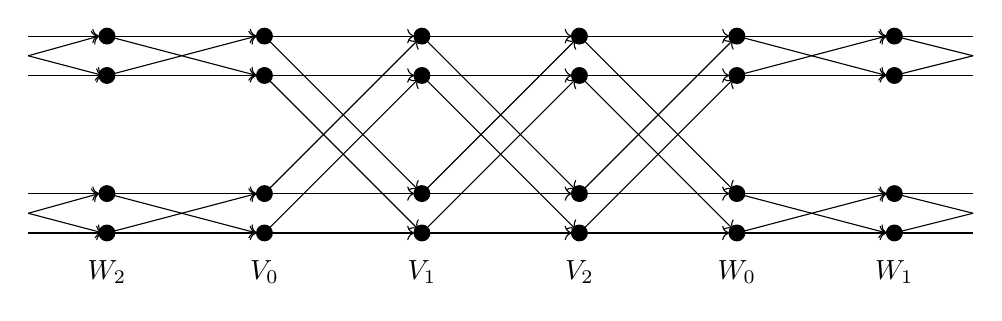
\begin{tikzpicture}[scale=0.5]

\begin{comment}
\draw (-4,4) circle (1);
\draw (-4,0) circle (1);
\draw (0,4) circle (1);
\draw (0,0) circle (1);
\draw (4,4) circle (1);
\draw (4,0) circle (1);
\draw (8,4) circle (1);
\draw (8,0) circle (1);
\draw (12,4) circle (1);
\draw (12,0) circle (1);
\draw (16,4) circle (1);
\draw (16,0) circle (1);
\end{comment}


\filldraw [black] (-4,4.5) circle (0.2);
\filldraw [black] (-4,3.5) circle (0.2);
\filldraw [black] (-4,0.5) circle (0.2);
\filldraw [black] (-4,-0.5) circle (0.2);
\filldraw [black] (0,4.5) circle (0.2);
\filldraw [black] (0,3.5) circle (0.2);
\filldraw [black] (0,0.5) circle (0.2);
\filldraw [black] (0,-0.5) circle (0.2);
\filldraw [black] (4,4.5) circle (0.2);
\filldraw [black] (4,3.5) circle (0.2);
\filldraw [black] (4,0.5) circle (0.2);
\filldraw [black] (4,-0.5) circle (0.2);
\filldraw [black] (8,4.5) circle (0.2);
\filldraw [black] (8,3.5) circle (0.2);
\filldraw [black] (8,0.5) circle (0.2);
\filldraw [black] (8,-0.5) circle (0.2);
\filldraw [black] (12,4.5) circle (0.2);
\filldraw [black] (12,3.5) circle (0.2);
\filldraw [black] (12,0.5) circle (0.2);
\filldraw [black] (12,-0.5) circle (0.2);
\filldraw [black] (16,4.5) circle (0.2);
\filldraw [black] (16,3.5) circle (0.2);
\filldraw [black] (16,0.5) circle (0.2);
\filldraw [black] (16,-0.5) circle (0.2);


\draw [->] (-4,4.5) -- (-0.2,4.5);
\draw [->] (-4,4.5) -- (-0.2,3.5);
\draw [->] (-4,3.5) -- (-0.2,4.5);
\draw [->] (-4,3.5) -- (-0.2,3.5);
\draw [->] (-4,0.5) -- (-0.2,0.5);
\draw [->] (-4,0.5) -- (-0.2,-0.5);
\draw [->] (-4,-0.5) -- (-0.2,0.5);
\draw [->] (-4,-0.5) -- (-0.2,-0.5);

\draw [->] (0,4.5) -- (4-0.2,4.5);
\draw [->] (0,4.5) -- (4-0.1,0.6);
\draw [->] (0,3.5) -- (4-0.2,3.5);
\draw [->] (0,3.5) -- (4-0.1,-0.4);
\draw [->] (0,0.5) -- (4-0.1,4.4);
\draw [->] (0,0.5) -- (4-0.2,0.5);
\draw [->] (0,-0.5) -- (4-0.1,3.4);
\draw [->] (0,-0.5) -- (4-0.2,-0.5);

\draw [->] (4,4.5) -- (8-0.2,4.5);
\draw [->] (4,4.5) -- (8-0.1,0.6);
\draw [->] (4,3.5) -- (8-0.2,3.5);
\draw [->] (4,3.5) -- (8-0.1,-0.4);
\draw [->] (4,0.5) -- (8-0.1,4.4);
\draw [->] (4,0.5) -- (8-0.2,0.5);
\draw [->] (4,-0.5) -- (8-0.1,3.4);
\draw [->] (4,-0.5) -- (8-0.2,-0.5);

\draw [->] (8,4.5) -- (12-0.2,4.5);
\draw [->] (8,4.5) -- (12-0.1,0.6);
\draw [->] (8,3.5) -- (12-0.2,3.5);
\draw [->] (8,3.5) -- (12-0.1,-0.4);
\draw [->] (8,0.5) -- (12-0.1,4.4);
\draw [->] (8,0.5) -- (12-0.2,0.5);
\draw [->] (8,-0.5) -- (12-0.1,3.4);
\draw [->] (8,-0.5) -- (12-0.2,-0.5);

\draw [->] (12,4.5) -- (16-0.2,4.5);
\draw [->] (12,4.5) -- (16-0.2,3.5);
\draw [->] (12,3.5) -- (16-0.2,4.5);
\draw [->] (12,3.5) -- (16-0.2,3.5);
\draw [->] (12,0.5) -- (16-0.2,0.5);
\draw [->] (12,0.5) -- (16-0.2,-0.5);
\draw [->] (12,-0.5) -- (16-0.2,0.5);
\draw [->] (12,-0.5) -- (16-0.2,-0.5);

\draw (16,4.5) -- (18,4.5);
\draw (16,4.5) -- (18,4);
\draw (16,3.5) -- (18,4);
\draw (16,3.5) -- (18,3.5);
\draw (16,0.5) -- (18,0.5);
\draw (16,0.5) -- (18,0);
\draw (16,-0.5) -- (18,0);
\draw (16,-0.5) -- (18,-0.5);

\draw [->] (-6,4.5) -- (-4.2,4.5);
\draw [->] (-6,4) -- (-4.1,3.5);
\draw [->] (-6,4) -- (-4.2,4.5);
\draw [->] (-6,3.5) -- (-4.1,3.5);
\draw [->] (-6,0.5) -- (-4.2,0.5);
\draw [->] (-6,0) -- (-4.1,-0.5);
\draw [->] (-6,0) -- (-4.2,0.5);
\draw [->] (-6,-0.5) -- (-4.1,-0.5);

\draw (-4,-1.5) node{$W_2$};
\draw (-0,-1.5) node{$V_0$};
\draw (4,-1.5) node{$V_1$};
\draw (8,-1.5) node{$V_2$};
\draw (12,-1.5) node{$W_0$};
\draw (16,-1.5) node{$W_1$};

\end{tikzpicture}
\caption{The graph $G_{\ell,m}$ when $\ell=4$ and $m=2$.}
\end{center}
\end{figure}

Assume for a contradiction that $G$ contains a $C_{\ell,\ell}$ composed of the two directed paths $x_0,\ldots,x_\ell$ and $y_0,\ldots,y_{\ell}$ where $x_0=y_0$ and $x_\ell=y_\ell$. By the symmetry of the $j$- and $k$-coordinates, we may assume that $x_0\in V_i$ for some $0\le i\le \ell-2$. Then $V(C_{\ell,\ell})\cap W_0=\{x_{\ell-1-i},y_{\ell-1-i}\}.$ Since $x_0=y_0$ and $x_{\ell-1-i}\ne y_{\ell-1-i}$, the structure of $G[V_0\cup\cdots V_{\ell-2}\cup W_0]$ guarantees that $x_{\ell-1-i}=w_{0jk}$ and $y_{\ell-1-i}=w_{0j'k}$ for some $j\ne j'$. Now $x_\ell\in W_{i+1}$ (with the convention $W_{\ell-1}=V_0$). Then the structure of $G[W_0,\ldots,W_{\ell-1}]$ implies that $x_\ell=w_{(i+1)jk'}$ and $y_\ell=w_{(i+1)j'k''}$ for some $k,k''$; but this contradicts $x_\ell=y_\ell$. 

Thus $G_{\ell,m}$ is a $C_{\ell,\ell}$-free digraph on $(2\ell-2)m^2$ vertices with minimum indegree and minimum outdegree $m$. This proves that for every $m$, $m^0((2\ell-2)m^2,C_{\ell,\ell})\ge m$. Given any $n\in\mathbb N$, there is some $n'$ of the form $n'=(2\ell-2)m^2$ with $n'\in(n,n +o(n))$. By applying Lemma \ref{density lemma}, we obtain
$$m^0(n,C_{\ell,\ell})\ge(1-o(1))\left\lfloor \left(\frac{n'}{2\ell-2}\right)^{1/2}\right\rfloor\ge\left(\frac{1}{(2\ell-2)^{1/2}}-o(1)\right)n^{1/2}.$$

The second inequality is immediate.

We now turn to the third inequality. Let $G$ be an $n$-vertex $C_{\ell,\ell}$-free graph with minimum outdegree $\delta^+$. Using \autoref{Removing short unbalanced cycles}, we pass to the directed graph $G'$ with $d:=\delta^+(G')\ge\frac{1-\varepsilon}{2\ell}\delta^+$ in which every closed walk of length at most $2\ell-1$ has type 0. Let $v\in V(G')$, and note there is a set $L_1$ of $d$ vertices in $N_{G'}^+(v)$. Assume we have constructed a set $L_i$ ($i\le\ell-2)$ of $d$ vertices such that
    for any $x,y\in L_i$ there are paths $P_1,P_2$ on $i$ edges oriented from $v$ to $x,y$ respectively so that 
    \begin{equation} \label{Path condition}
    V(P_1),V(P_2)\subseteq\{v\}\cup L_1\cup\cdots\cup L_{i}\text{ and }V(P_1)\cap V(P_2)=\{v\}.
    \end{equation}
    For $x\in L_i$ we have $|N^+(x)|\ge d$ so we can greedily choose distinct vertices $L_{i+1}=\{f(x):x\in L_i\}$ such that $(x,f(x))\in E(G')$ for all $x\in L_i$. Moreover we have $f(x)\not\in \{v\}\cup L_1\cup\cdots\cup L_i$ or else $G'$ would contain a cycle $C$ of length at most $2i+1$ with $t(C)\ne 0$, a contradiction. Thus, for $x,y\in L_i$ we can extend the paths $P_1$ and $P_2$ by the edges $(x,f(x)),(y,f(y))$ to satisfy \autoref{Path condition}. We arrive by induction at the set $L_{\ell-1}$. If there exist $x,y\in L_{\ell-1}$ and $z\in V(G')$ such that $(x,z),(y,z)\in E(G')$, then similarly to the above we have $z\not\in\{v\}\cup L_1\cup\cdots\cup L_{\ell-1}$. Thus, applying \autoref{Path condition} to the vertices $x,y$ and extending the paths by $xz,yz$ gives a copy of $C_{\ell,\ell}$, a contradiction. Hence $N^+_{G'}(x)\cap N_{G'}^+(y)=\emptyset$ so 
    $$n\ge\left|\bigcup_{x\in L_{\ell-1}}N_{G'}^+(x)\right|\ge d\cdot d$$
    which gives 
    $\left(\frac{1-\varepsilon}{2\ell}\delta^+\right)^2\le n$ and the result follows.
\qed

\subsection{Proof of \autoref{Path separation application}}

    Let $\ell=2r$. Assume for the time being that $(2r-2)(2r+1)|n$. First we count Hamilton cycles in the graph $G=G_{r,m}$ from \autoref{Glm definition} with $m^2=n/(2r-2)$. Note that $G[V_0,\ldots,V_{\ell-1}]$ and $G[W_0,\ldots,W_{\ell-1}]$ are each $m$ disjoint copies of a blowup of a directed $P_{\ell-1}$. Let $X_1,\ldots,X_m$ be the components of $G[V_0,\ldots,V_{\ell-1}]$ and let $Y_1,\ldots,Y_m$ be the components of $G[W_0,\ldots,W_{\ell-1}]$.   A \textit{transition vector} is a word
$$t=X_{f(1)}Y_{g(1)}X_{f(2)}Y_{g(2)}\ldots X_{f(m^2)}Y_{g(m^2)}$$
with properties
\begin{itemize}
    \item $f,g:[m^2]\to[m]$
    \item for each $i,j\in[m]$, the contiguous subwords $X_iY_j$ and $Y_jX_i$ each occur exactly once (we consider the vector cyclically, so that $Y_{f(m^2)}X_{f(1)}$ is a contiguous subword).
    \item $f(1)=g(1)=1$.
\end{itemize}
(The importance of the second property comes from the fact that, for any $X_i$ and $Y_j$, there are exactly two vertices in $X_i\cap Y_j$, one in $V_0$ and one in $W_0$. As we will see below, the second property is used to guarantee that certain walks associated with the transition vector visit each vertex in $V_0\cup W_0$ exactly once.) A transition vector is equivalent to an Eulerian circuit in the bidirected $K_{m,m}$. To enumerate Eulerian circuits we refer to the famous result of de Bruijn, van Aardenne-Ehrenfest, Smith, and Tutte.
\begin{thm}[BEST \cite{van1987circuits}]
Let $G$ be a strongly connected digraph in which every vertex $v$ has $d^+(v)=d^-(v)$. Let $t_v(G)$ denote the number of oriented spanning subtrees with root $v$. Then for any $v\in V(G)$ the number of Eulerian circuits of $G$ is
$$\mathrm{ec}(G)=t_v(G)\prod_{v\in V(G)}(d^+(v)-1)!.$$
\end{thm}
There are $m^{2(m-1)}$ spanning trees of $K_{m,m}$ \cite{moh1990number}, so we conclude that there are $m^{2(m-1)}(m-1)!^{2m}$ transition vectors.
We say that a Hamilton cycle
$$H=v_{0j_1k_1}\cdots w_{0j_2k_1}\cdots v_{0j_2k_2}\cdots w_{0j_3k_2}\cdots\cdots v_{0j_1k_1}$$
(making no assumptions on the hidden portions of the vertex sequence) \textit{follows} the transition vector $t$ if $v_{0j_sk_s}\in X_{f(s)}$ and $w_{0j_{s+1}k_s}\in Y_{g(s)}$ for every $s\in[m^2]$, i.e. $k_s=f(s)$ and $j_{s+1}=g(s)$ (see \autoref{Hamilton cycle figure}).

\begin{claim} \label{Hamilton cycles following t}
For any transition vector $t$ there are exactly $(m!)^{2m(r-2)}$ Hamilton cycles in $G$ which follow $t$.
\end{claim}
\begin{proof}
    We consider any component $X_i$ of $G[V_0,\ldots,W_0]$. Each time a Hamilton path $H$ which follows $t$ visits a vertex $v\in V_0\cap X_i$, we must choose a path in $X_i$ from $v$ to the unique vertex $w\in W_0\cap Y_j$ where $Y_j$ is the component indicated by $t$ via the subword $X_iY_j$. (We know $w$ is unvisited since if it was visited previously then $X_iY_j$ must have already occurred in $t$, as $X_i\cap Y_j\cap W_0=\{w\}$.) The first time that $V_0\cap X_i$ is visited there are $m^{r-2}$ choices for such a path (only the last edge is forced), the second time there are $(m-1)^{r-2}$ choices, and so on, so that varying the paths taken inside $X_i$ gives $m^{r-2}\cdots 1^{r-2}=(m!)^{r-2}$ total choices. Similarly there are $(m!)^{r-2}$ total choices for the paths inside each $Y_j$, so considering all components together we arrive at $((m!)^{r-2})^{2m}$ Hamilton paths.
\end{proof}

\begin{figure}[h] 
\begin{center}

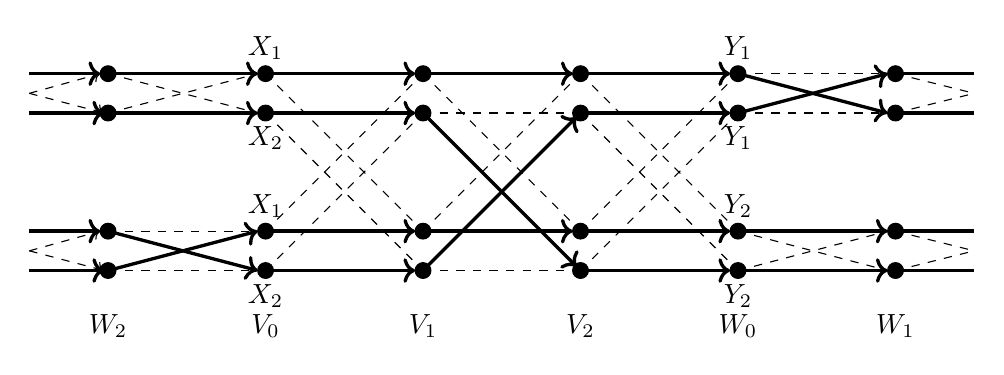
\begin{tikzpicture}[scale=0.5]

\filldraw [black] (-4,4.5) circle (0.2);
\filldraw [black] (-4,3.5) circle (0.2);
\filldraw [black] (-4,0.5) circle (0.2);
\filldraw [black] (-4,-0.5) circle (0.2);
\filldraw [black] (0,4.5) circle (0.2);
\draw [above] (0,4.6) node{$X_1$};
\filldraw [black] (0,3.5) circle (0.2);
\draw [below] (0,3.4) node{$X_2$};
\filldraw [black] (0,0.5) circle (0.2);
\draw [above] (0,0.6) node{$X_1$};
\filldraw [black] (0,-0.5) circle (0.2);
\draw [below] (0,-0.6) node{$X_2$};
\filldraw [black] (4,4.5) circle (0.2);
\filldraw [black] (4,3.5) circle (0.2);
\filldraw [black] (4,0.5) circle (0.2);
\filldraw [black] (4,-0.5) circle (0.2);
\filldraw [black] (8,4.5) circle (0.2);
\filldraw [black] (8,3.5) circle (0.2);
\filldraw [black] (8,0.5) circle (0.2);
\filldraw [black] (8,-0.5) circle (0.2);
\filldraw [black] (12,4.5) circle (0.2);
\draw [above] (12,4.6) node{$Y_1$};
\filldraw [black] (12,3.5) circle (0.2);
\draw [below] (12,3.4) node{$Y_1$};
\filldraw [black] (12,0.5) circle (0.2);
\draw [above] (12,0.6) node{$Y_2$};
\filldraw [black] (12,-0.5) circle (0.2);
\filldraw [black] (16,4.5) circle (0.2);
\draw [below] (12,-0.6) node{$Y_2$};
\filldraw [black] (16,3.5) circle (0.2);
\filldraw [black] (16,0.5) circle (0.2);
\filldraw [black] (16,-0.5) circle (0.2);


\draw [very thick,->] (-4,4.5) -- (-0.2,4.5);
\draw [dashed] (-4,4.5) -- (-0.2,3.5);
\draw [dashed] (-4,3.5) -- (-0.2,4.5);
\draw [very thick,->] (-4,3.5) -- (-0.2,3.5);
\draw [dashed] (-4,0.5) -- (-0.2,0.5);
\draw [very thick,->] (-4,0.5) -- (-0.2,-0.5);
\draw [very thick,->] (-4,-0.5) -- (-0.2,0.5);
\draw [dashed] (-4,-0.5) -- (-0.2,-0.5);

\draw [very thick,->] (0,4.5) -- (4-0.2,4.5);
\draw [dashed] (0,4.5) -- (4-0.1,0.6);
\draw [very thick,->] (0,3.5) -- (4-0.2,3.5);
\draw [dashed] (0,3.5) -- (4-0.1,-0.4);
\draw [dashed] (0,0.5) -- (4-0.1,4.4);
\draw [very thick,->] (0,0.5) -- (4-0.2,0.5);
\draw [dashed] (0,-0.5) -- (4-0.1,3.4);
\draw [very thick,->] (0,-0.5) -- (4-0.2,-0.5);

\draw [very thick,->] (4,4.5) -- (8-0.2,4.5);
\draw [dashed] (4,4.5) -- (8-0.1,0.6);
\draw [dashed] (4,3.5) -- (8-0.2,3.5);
\draw [very thick,->] (4,3.5) -- (8-0.1,-0.4);
\draw [dashed] (4,0.5) -- (8-0.1,4.4);
\draw [very thick,->] (4,0.5) -- (8-0.2,0.5);
\draw [very thick,->] (4,-0.5) -- (8-0.1,3.4);
\draw [dashed] (4,-0.5) -- (8-0.2,-0.5);

\draw [very thick,->] (8,4.5) -- (12-0.2,4.5);
\draw [dashed] (8,4.5) -- (12-0.1,0.6);
\draw [very thick,->] (8,3.5) -- (12-0.2,3.5);
\draw [dashed] (8,3.5) -- (12-0.1,-0.4);
\draw [dashed] (8,0.5) -- (12-0.1,4.4);
\draw [very thick,->] (8,0.5) -- (12-0.2,0.5);
\draw [dashed] (8,-0.5) -- (12-0.1,3.4);
\draw [very thick,->] (8,-0.5) -- (12-0.2,-0.5);

\draw [dashed] (12,4.5) -- (16-0.2,4.5);
\draw [very thick,->] (12,4.5) -- (16-0.2,3.5);
\draw [very thick,->] (12,3.5) -- (16-0.2,4.5);
\draw [dashed] (12,3.5) -- (16-0.2,3.5);
\draw [very thick,->] (12,0.5) -- (16-0.2,0.5);
\draw [dashed] (12,0.5) -- (16-0.2,-0.5);
\draw [dashed] (12,-0.5) -- (16-0.2,0.5);
\draw [very thick,->] (12,-0.5) -- (16-0.2,-0.5);

\draw [very thick] (16,4.5) -- (18,4.5);
\draw [dashed] (16,4.5) -- (18,4);
\draw [dashed] (16,3.5) -- (18,4);
\draw [very thick] (16,3.5) -- (18,3.5);
\draw [very thick] (16,0.5) -- (18,0.5);
\draw [dashed] (16,0.5) -- (18,0);
\draw [dashed] (16,-0.5) -- (18,0);
\draw [very thick] (16,-0.5) -- (18,-0.5);

\draw [very thick,->] (-6,4.5) -- (-4.2,4.5);
\draw [dashed,->] (-6,4) -- (-4.1,3.5);
\draw [dashed,->] (-6,4) -- (-4.2,4.5);
\draw [very thick,->] (-6,3.5) -- (-4.1,3.5);
\draw [very thick,->] (-6,0.5) -- (-4.2,0.5);
\draw [dashed,->] (-6,0) -- (-4.1,-0.5);
\draw [dashed,->] (-6,0) -- (-4.2,0.5);
\draw [very thick,->] (-6,-0.5) -- (-4.1,-0.5);

\draw (-4,-1.9) node{$W_2$};
\draw (-0,-1.9) node{$V_0$};
\draw (4,-1.9) node{$V_1$};
\draw (8,-1.9) node{$V_2$};
\draw (12,-1.9) node{$W_0$};
\draw (16,-1.9) node{$W_1$};

\end{tikzpicture}
\caption{The solid lines describe a Hamilton cycle in $G_{4,2}$ which follows the transition vector $X_1Y_1X_2Y_2X_1Y_2X_2Y_1$.} \label{Hamilton cycle figure}
\end{center}
\end{figure}

Note that every Hamilton cycle follows exactly one transition vector. Therefore, the number of Hamilton cycles in $G$ is
$$\begin{aligned}m^{2(m-1)}(m-1)!^{2m}m!^{2m(r-2)}=m^{(2r-2)m^2+O(m^2/\log m)}=n^{n/2+O(n/\log n)}.\end{aligned}$$

It follows there is a family $\mathcal P$ of $n^{n/2+O(n/\log n)}$ Hamilton paths in $G$. Suppose $P,Q\in\mathcal P$ and $P\cup Q$ contains a 2-part $\ell$-cycle $C$. Since $G_{r,m}$ contains no $C_{r,r}$, and $C_{r,r}$ is the unique 2-part cycle of type 0, we have $t(C)\ne 0$. We will filter out these remaining $\ell$-cycles. Partition $[n]$ into equal parts $N=N_0\sqcup\cdots\sqcup N_{2r}$. Let $\Sigma$ be the set of all Hamilton paths starting in $N_0$ and whose $i^{th}$ vertex belongs to $N_{i\pmod{2r+1}}.$ Clearly no two paths in $\Sigma$ create an unbalanced $\ell$-cycle, and
    $$|\Sigma|=\left(\frac{n}{2r+1}\right)^{2r+1}\left(\frac{n}{2r+1}-1\right)^{2r+1}\cdots(1)^{2r+1}=(n/(2r+1))!^{2r+1}=n^{n+O(n/\log n)}.$$
Let $\pi$ be a random relabeling of $[n]$, then taking an outcome in which $|\pi\mathcal P\cap\Sigma|$ is at least average, we obtain a family $\mathcal P'$ of Hamilton paths no two of which create any two-part cycle, with $|\mathcal P'|=n^{n/2+O(n/\log n)}$. To convert this to an upper bound on $\hat M(n,\ell)$ we refer to a folklore lemma about vertex-transitive graphs (see e.g. \cite{godsil2001algebraic}, Lemma 7.2.2) 
\begin{lemma} \label{Vertex transitive lemma}
If a graph $G$ is vertex-transitive, then
$$\alpha(G)\omega(G)\le|V(G)|.$$
\end{lemma}
 Consider the graph whose vertices are Hamilton paths on $[n]$ where two paths are adjacent if they create a two-part $\ell$-cycle. Then $\mathcal{P}'$ corresponds to an independent set. Applying \autoref{Vertex transitive lemma} to this graph, we obtain $$\hat M(n,\ell)\le\frac{n!}{n^{n/2+O(n/\log n)}}=(n!)^{1/2+O(1/\log n)}.$$
Now consider general $n\in\mathbb N$. Note that $\hat M(n,\ell)$ is increasing. Thus taking the smallest $n'>n$ satisfying $(2r-2)(2r+1)|n'$ gives
$$\hat M(n,\ell)\le (n+O(1))!^{1/2+O(1/\log n)}=(n!)^{1/2+O(1/\log n)}.$$
\qed



\section{Concluding remarks} \label{Concluding remarks}

\begin{comment}
Unfortunately \autoref{hamilton cycles result} is not strong enough to prove an upper bound on $\mathrm{ex}(n,\{C_3,\ldots,C_{2k}\})$ in terms of $M_k(S_n)$, since we require a pseudorandomness property in order to obtain many Hamilton cycles. However, it seems plausible that the pseudorandomness property could be relaxed to something like regularity since being the permutations being cyclic is much stronger than what is actually required for the proof to work, namely that they have no 1- or 2-cycles in their disjoint cycle decomposition. \john{rephrase or remove}
\end{comment}

\begin{comment}
We considered whether \autoref{second kind result} generalizes to forbid equations of the form
$$\alpha_1\beta_1^{-1}\cdots\alpha_k\beta_k^{-1}=1$$
where $\alpha_i\ne\beta_i\ne\alpha_{i+1}$. The analysis of the condition
$$\forall i\ (\alpha_1\beta^{-1}\cdots\alpha_k\beta_k^{-1})(i)=i$$
seems to become complicated when $k\ge 3$, and we do not know whether a connection to the function $\Delta^{2k}_v(n)$ (for some $v\le 2k$) could be obtained.
\end{comment}

As noted in \autoref{Introduction}, taking all matchings in a $C_4$-free bipartite graph does not give rise to an $S_2'$-set in the symmetric group. Instead, it obtains a family $\mathcal F$ of permutations satisfying the weaker condition that for all $\alpha,\beta,\gamma,\delta\in\mathcal F$, 
    \begin{equation} \label{sidon implication}
    \alpha\beta^{-1}=\gamma\delta^{-1}\Longrightarrow\forall i\ [\alpha(i)=\beta(i)\text{ and }\gamma(i)=\delta(i)]\text{ or }[\alpha(i)=\gamma(i)\text{ and }\beta(i)=\delta(i)].
    \end{equation}
We attempted to improve \autoref{Probabilistic constructions} in the case $\Gamma=S_n$ by intersecting $\mathcal F$ with a family $\mathcal G\subseteq S_n$ such that for all distinct $\alpha,\beta,\gamma,\delta\in\mathcal G$ there exists $i\in[n]$ such that $|\{\alpha(i),\beta(i),\gamma(i),\delta(i)\}|\ge 3$. However, Bukh and Keevash \cite{Bukh2025generalization} proved the following theorem that generalizes the upper bound of Blackburn and Wild \cite{blackburn1998optimal} on perfect hash codes.

%that if $S\subseteq[q]^n$ is a family of words such that for any $t$ of the words there exists a coordinate on which they attain at least $v$ distinct values, then $|S|\le {t\choose 2}q^{\left(1-\frac{v-2}{t-1}\right)n}$ (this generalizes the upper bound of Blackburn and Wild \cite{blackburn1998optimal} on perfect hash codes.) 

\begin{thm}[Bukh and Keevash \cite{Bukh2025generalization}]\label{BK theorem}
Suppose that $S\subseteq [q]^n$ is family of words such that among every $t$ words there is a coordinate
with at least $v$ values. Then $|{S}|\leq \binom{t}{2}q^{(1-\frac{v-2}{t-1})n}$.
\end{thm}
Before proving the theorem, a lemma is needed.
\begin{lemma}\label{fam}
  There is a family $\mathcal{F}\subset \binom{[t-1]}{v-2}$ of size $|{\mathcal{F}}|=t-1$ such that every element of $[t-1]$
  is in exactly $v-2$ sets of $\mathcal{F}$.
\end{lemma}
\begin{proof}
Let $\mathcal{F}$ consist of cyclic shifts of $[v-2]$ modulo $t-1$.
\end{proof}
\begin{proof}[Proof of Theorem \ref{BK theorem}]
Let $\mathcal{F}=\{I_1,\dotsc,I_{t-1}\}$ be the family as in Lemma \ref{fam}. Cut each word $w\in S$ into $t-1$ consecutive subwords $w_1,...,w_{t-1}$ of length
$n/(t-1)$ each. For a set $I\in \mathcal{F}$, define $w_I$ to be the
concatenation of the words $(w_i)_{i \in [t-1]\setminus I}$. So, $w_I$ is a word of length
$(1-\frac{v-2}{t-1})n$.

Do the following for as long as possible: if there is a pair $(j,u)\in [t-1]\times [q]^{(1-\frac{v-2}{t-1})n}$ such that
the set $S_{j,u}:= \{w\in S: w_{I_j}=u\}$ has at most $j$ elements, remove all elements of $S_{j,u}$ from $S$. Note
that each pair $(j,u)$ occurs at most once in this process. So, the total number of words removed from $S$ is
at most $\binom{t}{2}q^{(1-\frac{v-2}{t-1})n}$.

We claim that $S$ is now empty. Indeed, suppose that some word $w$ survived to the end of this process.
For each $j=1,2,\dotsc,t-1$ in order, find a word $w^{(j)}\in S$ such that $w^{(j)}_{I_j}=w_{I_j}$ and such that
$w^{(j)}$ is distinct from previously selected words $w,w^{(1)},\dotsc,w^{(j-1)}$. The latter is possible because survival of $w$ implies
$|{S_{j,w_{I_j}}}|>j$.

The definition of $\mathcal{F}$ implies that in each coordinate the $t$ words $w,w^{(1)},\dotsc,w^{(t-1)}$ take at most $v-1$ values.
As the words are distinct, we reached a contradiction.
\end{proof}


This implies that our approach only proves that $M_2'(S_n)\ge(n!)^{1/6+O(1/\log n)}$. We believe that such `$t$-wise $v$-different codes' may be of some independent interest.

We considered whether the idea in our construction of $S_2$-sets in $S_n\times S_n$ could be generalized to give $S_2'$-sets or to give $S_k$-sets for $k\ge 3$. For $S_2'$-sets, we looked for constructions taken from the set $B=\{(f(\alpha),g(\alpha)):\alpha\in S_n\}$, where $f(\alpha)$ and $g(\alpha)$ are some words on $\alpha$ and some fixed permutations. It seems to us that for any choice of $f,g$, the equations of the form $x_1y_1^{-1}x_2y_2^{-1}=1$ with variables in $B$ either simplify to a single Sidon equation in $S_n$, or are too complicated to usefully employ the choice of $f,g$. We were also unable to find any similar construction that works for $S_k$-sets ($k\ge 3$). It may be interesting to see whether there is a natural construction of $S_k$-sets in $S_n^k$, extending our loose analogy with the abelian constructions.

Besides the constructions used in \autoref{Sn times Sn result} we found other $S_2$-sets of the same size. Let $\pi',\sigma'$ be two permutations of $[n]$ such that $\pi:=(\pi')^2,\sigma:=(\sigma')^2$ are both derangements and involutions, and such that $\sigma\pi=\rho_1\rho_2$ for two disjoint $(n/2)$-cycles $\rho_1,\rho_2$. Then one can show that $\{(\pi'\alpha\pi',\sigma'\alpha\sigma'):\alpha\in S_n,\alpha(1)=1\}$ is an $S_2$-set in $S_n\times S_n$, and in fact it is also a special case of \autoref{recipe}.

It is interesting that the proof of \autoref{Sk upper bound} does not work when $k$ is odd. In fact, if $k=2r+1$ then as in the proof of \autoref{Sk upper bound} one can define $L=\{\alpha_1\cdots\alpha_{r+1}:\alpha_i\in A\}$ and show that $L$ is a near-optimal $S_2[|A|]$-set. However, when $g\ge 2$ it is possible for large $S_2[g]$-sets to exist in abelian groups, so only the final step in the proof fails.

We list some open questions:
\begin{itemize}
    \item[(1)] %Does there exist $c>0$ such that
    %$$M_k(\Gamma)\ge c|\Gamma|^{1/k}$$ 
    %for every finite nonabelian group $\Gamma$? \john{no: $k=2$, $\Gamma$ is the dihedral group} \john{really this question is about whether there is a sequences of groups such that 
    %$$\omega(1)\le M_k(\Gamma)\le o(|\Gamma|^{1/k}).$$}
    For each $k\ge2$ do there exist constants $C,c$ such that
    $$M_k(\Gamma)\le C\text{ or }M_k(\Gamma)\ge c|\Gamma|^{1/k}$$
    holds for every finite group $\Gamma$?
    \item[(2)] Does \autoref{Sk upper bound} extend to the case that $k$ is odd?
    \item[(3)] Improve the lower or upper bounds in the inequalities
    $$(n!)^{1/k-O(1/\log n)}\le M_k(S_n)<(n!)^{1/k}$$
    and
    $$(n-1)!\le M_2(S_n\times S_n)<n!.$$
\end{itemize}

\section{Acknowledgements}

The authors would like to thank Boris Bukh and Peter Keevash for the proof of Theorem \ref{BK theorem}. This research was partially supported by NSF DMS-2245556.

%\printbibliography

\bibliographystyle{plain}
	\bibliography{references.bib}

\end{document}
